\noindent

\includegraphics[height=1.25cm]{images/pictograms/replication}

\includegraphics[height=1.25cm]{images/pictograms/benchmark}

\includegraphics[height=1.25cm]{images/pictograms/tools}

\includegraphics[height=1.25cm]{images/pictograms/FDM}

\includegraphics[height=1.25cm]{images/pictograms/3d}

\includegraphics[height=1.25cm]{images/pictograms/paraview}

%%%%%%%%%%%%%%%%%%%%%%%%%%%%%%%%%%%%%%%%%%%%%%%%%%%%%%%%%%%%%%%%%%%%%%%%%%%%%%%%%%%%%%%%%%%%%%%%%%%

\begin{flushright} {\tiny {\color{gray} python\_codes/fieldstone\_171/text.tex}} \end{flushright}

%\lstinputlisting[language=bash,basicstyle=\small]{python_codes/template_keywords.key}

\par\noindent\rule{\textwidth}{0.4pt}

\begin{center}
\inpython
{\small Code: \url{https://github.com/cedrict/fieldstone/tree/master/python_codes/fieldstone_171}}
\end{center}

\par\noindent\rule{\textwidth}{0.4pt}

{\sl This stone was developed with input from L. van de Wiel}. \index{contributors}{L. van de Wiel}

\par\noindent\rule{\textwidth}{0.4pt}

Last revision: April 6th, 2025.

\par\noindent\rule{\textwidth}{0.4pt}

%%%%%%%%%%%%%%%%%%%%%%%%%%%%%%%%%%%%%%%%%%%%%%%%%%%%%%%%%%%%%%%%%%%%%%%%%%%%%%%%%%%%%%%%%%%%%%%%%%%

There is a lot of literature and online material about these equations. I make use of the following 
ones in what follows:
\begin{itemize}
\item \fullcite{grsc84}
\item \fullcite{pear93}
\item \fullcite{lemo93}
\item \fullcite{haqh16} (they talk about blob detection and shannon entropy. Explore?)
\item \fullcite{muna14}
\item \fullcite{gane22}
\item \fullcite{gama23}
\item \url{http://www.mrob.com/pub/comp/xmorphia/index.html} by R. Munafo
\item \url{https://en.wikipedia.org/wiki/Reaction-diffusion_system}
\end{itemize}

The Gray–Scott reaction–diffusion system of equations are given by
\begin{eqnarray}
\frac{\partial u}{\partial t} &=& D_u \vec\nabla^2 u - uv^2 + F(1-u) \nn\\
\frac{\partial v}{\partial t} &=& D_v \vec\nabla^2 v + uv^2 - (F+k)v
\end{eqnarray}
where $D_u$ and $D_v$ are diffusion coefficients associated with the species concentration $u$
and $v$. $k$ is the dimensionless rate constant of the second reaction (also commonly called the `kill 
parameter') and $F$ is the dimensionless feed rate.
Often periodic boundary conditions are used. 

In his 1993 landmark paper \textcite{pear93} reveals a surprising variety of 
irregular spatiotemporal patterns as shown in Fig. 2\&3 of the paper:

\begin{center}
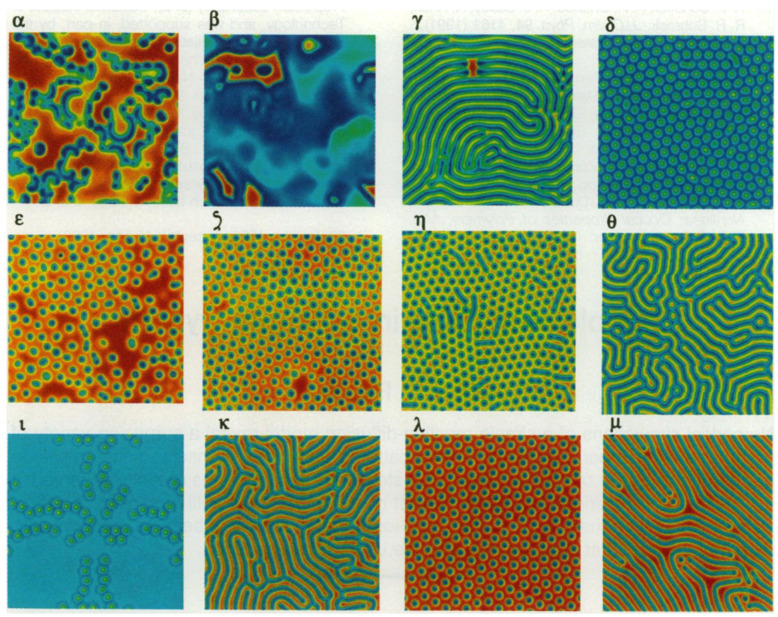
\includegraphics[height=7.5cm]{python_codes/fieldstone_171/images/pear93a}
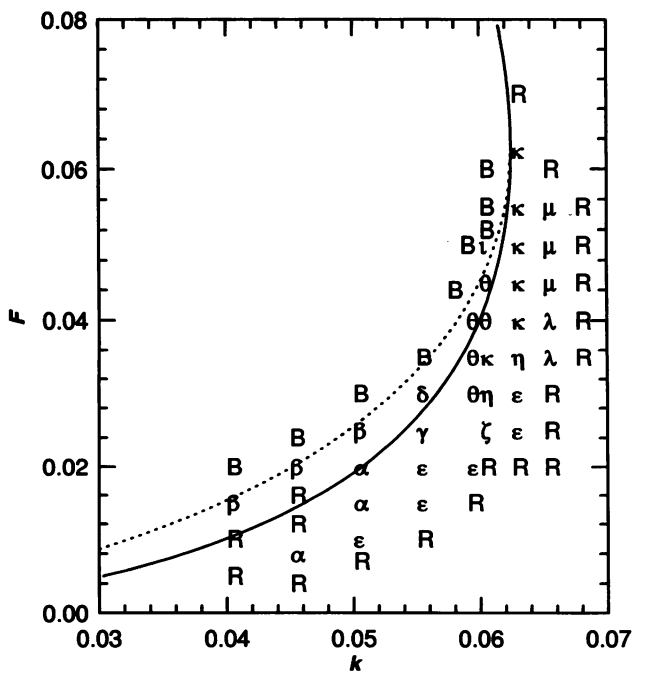
\includegraphics[height=7.5cm]{python_codes/fieldstone_171/images/pear93b}\\
{\captionfont Taken from \cite{pear93}. Left: The key to the map. The patterns 
shown in the figure are designated by Greek letters, which are used in 
[the right figure] to indicate the pattern found at a given point in parameter space.
Right: The Greek letters indicate the location in parameter
space where the patterns in [the left figure] were found; B and R indicate that
the system evolved to uniform blue and red states, respectively.
} 
\end{center}

In the paper the domain is a square of size $L=2.5$ with $D_u=2\cdot 10^{-5}$
and $D_v=10^{-5}$. The boundary conditions are periodic.
The simulations are forward Euler integrations of the finite-difference equations 
resulting from discretization of the diffusion operator (or, FTCS). 
The spatial mesh consists of 256 by 256
grid points. The time step used is 1. Spot checks made with meshes as large as 1024 by
1024 and time steps as small as 0.01 produced no qualitative difference in the results.

Initially, the entire system was placed in the trivial state ($u=1,v=0$). The 20 by
20 mesh point area located symmetrically about the center of the grid was then
perturbed to ($u=1/2,v=1/4$). These conditions were then perturbed with $\pm 1\%$
random noise in order to break the square symmetry. The system was then integrated
for 200,000 time steps. 

Depending on the parameter values, it took on the order of 10,000 to
20,000 time steps for the initial perturbation to spread over the entire grid. 
After the initial period during which the perturbation spread, 
the system went into an asymptotic state that was either
time-independent or time-dependent, depending on the parameter values.

Likewise in \textcite{gane22} (2022) we find the following figure:
\begin{center}
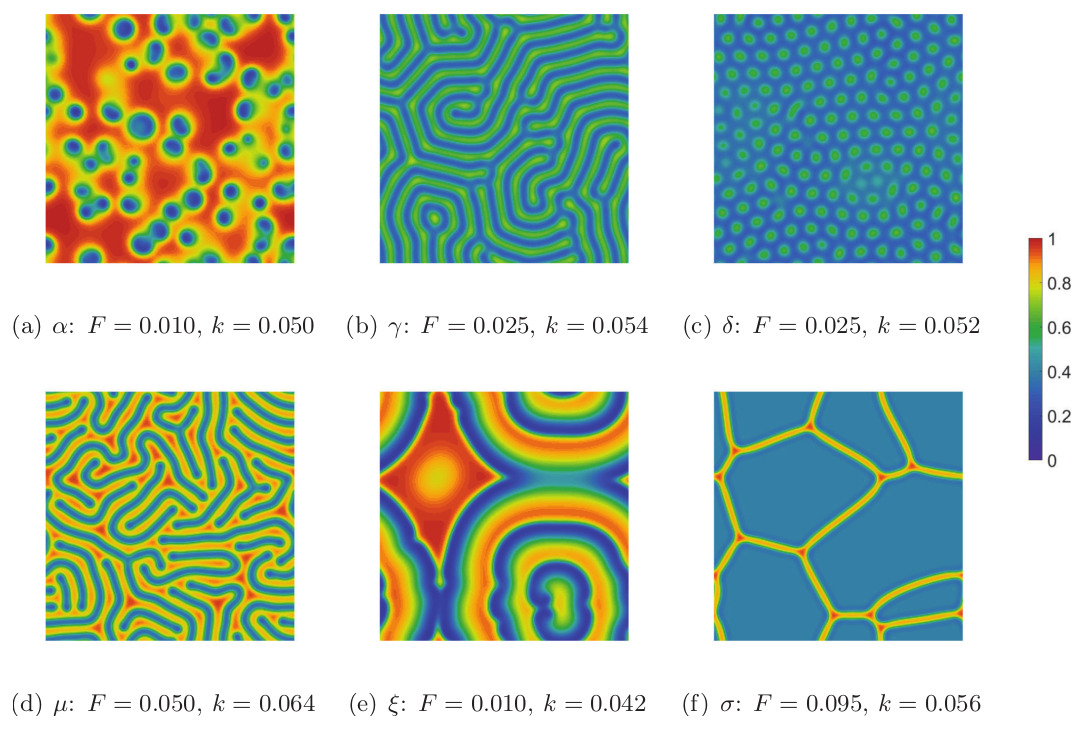
\includegraphics[height=7.5cm]{python_codes/fieldstone_171/images/gane22}\\
{\captionfont Taken from \cite{gane22}. 
Snapshots of a selection of two-dimensional patterns obtained for
$D_u=2\cdot 10^{-5}$ and $D_v=1\cdot 10^{-5}$ obtained via numerical 
simulation in MATLAB. Patterns are classified according to the Greek letter 
naming convention used by \textcite{pear93}.
} 
\end{center}

%%%%%%%%%%%%%%%%%%%%%%%%%%%%%%%%%%%%%%%%%%%%%%%%%%%%
\section*{About the work of R. Munafo}

We find on his website\footnote{\url{http://www.mrob.com/pub/comp/xmorphia/pearson-classes.html}}
two key figures:

\begin{center}
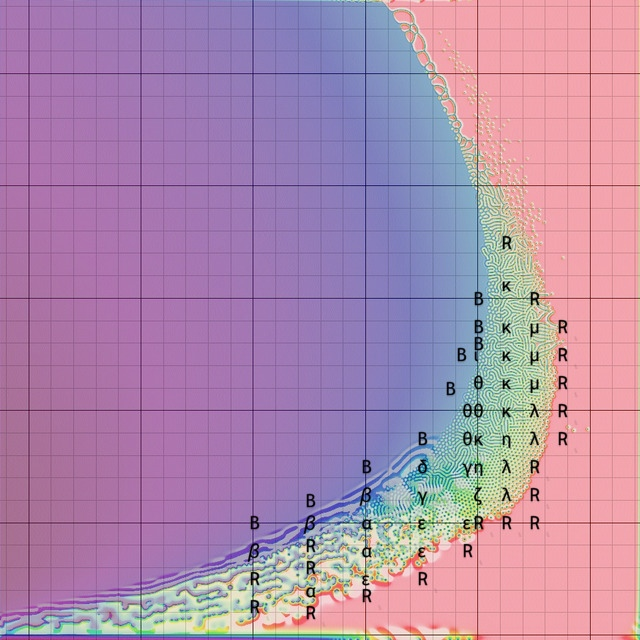
\includegraphics[height=7.5cm]{python_codes/fieldstone_171/images/pearson-orig}
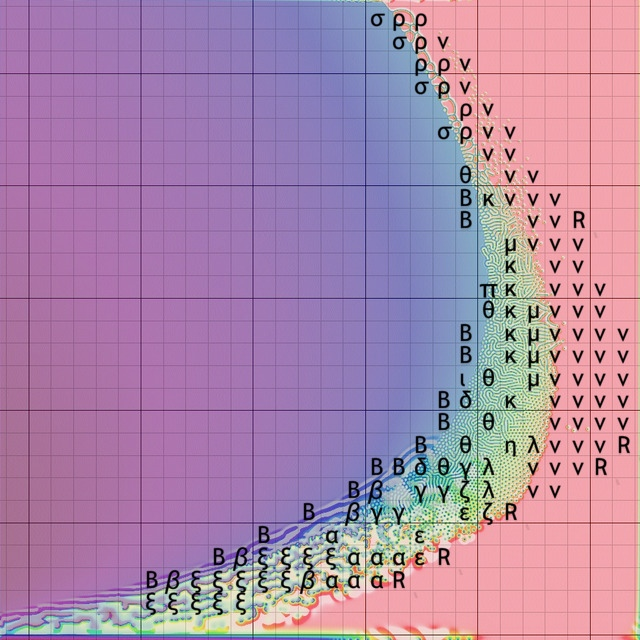
\includegraphics[height=7.5cm]{python_codes/fieldstone_171/images/pearson-tags}\\
{\captionfont So called key maps of the Gray-Scott equations. $k$ is on the 
horizontal axis, $F$ is on the vertical axis. Thick lines correspond to 
0.2-0.7 on the x-axis and to 0.3-0.8 on the y-axis.
The classification of the solution is traditionally based on Greek letters:
alpha ($\alpha$),    beta ($\beta$),    gamma ($\gamma$),    delta ($\delta$),    
epsilon ($\epsilon$),    zeta ($\zeta$),    eta ($\eta$),    
theta ($\theta$),    iota ($\iota$),    kappa ($\kappa$),    lambda ($\lambda$),    
mu ($\mu$),    nu ($\nu$),    xi ($\xi$),    pi ($\pi$),    rho ($\rho$),    sigma ($\sigma$).
The first fourteen
(R, B, and $\alpha$ through $\mu$) were defined by Pearson \cite{pear93} (left figure); 
On the right we find the data from his figure 3 (with corrections) replotted on the index image from the left figure. 
}
\end{center}

It is interesting to note that the greek letters on the left figure are
not exactly coinciding with those of the original paper...

The author further states:
\begin{displayquote}
{\color{darkgray}
Pearson missed many types of patterns because he only used one starting pattern: 
a small $(u,v)=(1/2,1/4)$ square on an otherwise (1,0) background. Many combinations 
of parameters $(F,k)$ fail to produce 
a pattern if initialised this way, but produce patterns when started some other way 
(such as a single small spot on 
an otherwise (0, 1) background, resembling the inverse of Pearson's initialisation; or several spots of
diverse $(F,k)$ values). 
Types nu, xi, pi, rho, and sigma are of this sort and were identified by me; 
the first three of these are described in my paper [2]. 
Types rho, and sigma also require a model with somewhat higher 
resolution than Pearson's, and significantly better runtime; these requirements would have made their discovery 
nearly impossible in the 1990s.
}
\end{displayquote} 




%%%%%%%%%%%%%%%%%%%%%%%%%%%%%%%%%%%%%%%%%%%%
%\section*{}
\textcite{gama23} (2023) rely on these equations to generate porous geometries 
and the following values of $D_u,D_v,f,k$ are used:

\begin{center}
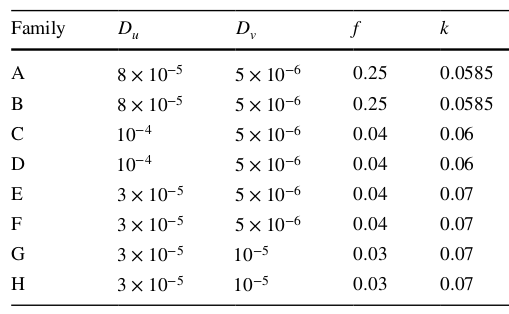
\includegraphics[width=6cm]{python_codes/fieldstone_171/images/gama01}
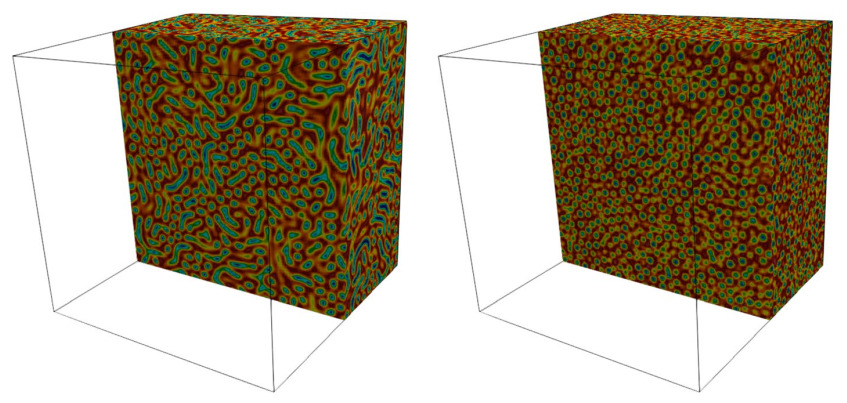
\includegraphics[width=9cm]{python_codes/fieldstone_171/images/gama02}\\
{\captionfont Iso-surfaces for solutions to the reaction-diffusion system 
for two set of parameters $\{D_u,D_v,F,k\}$, the parameters on the figure on 
the left(right) correspond to family A/B(C/D) in the table. The solutions were
obtained on a cube of length $L=192$.}
\end{center}

In the articles the authors use spherical initial distributions given by:
\begin{eqnarray}
U(r,\theta,\phi) &=& H_e(r-r_c) +\frac12 (1-H_e(r-r_c)) + 0.01 \cdot {\cal U}_{[0,1]} \nn\\
V(r,\theta,\phi) &=& \frac14 (1-H_e(r-r_c)) + 0.01 \cdot {\cal U}_{[0,1]}
\end{eqnarray}
where $H_e$ is the Heaviside step function, ${\cal U}_{[0,1]}$ is a random variable sourced from a 
uniform distribution defined between $[0,1]$, and $(r,\theta,\phi)$ are spherical coordinates centered at
the cube center, and $r_c$ is a constant (5 or 7).
The equations are solved numerically via a finite difference scheme on a square/cube of size $L$
with periodic boundary conditions. As time evolves, the patterns generated by
the solutions reveal a class of solutions whose iso-surfaces are reminiscent of the internal
boundaries encountered on porous media as shown in the figure above.

\textcite{haqh16} (2016) also investigate pattern formation:
\begin{center}
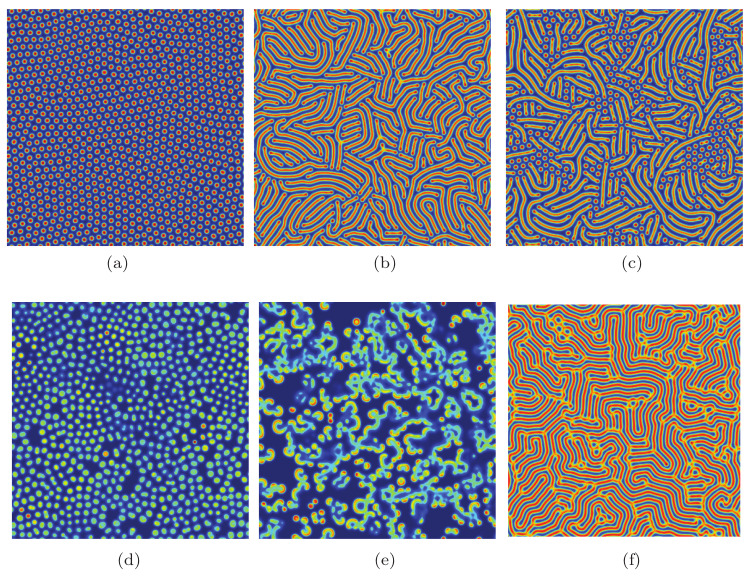
\includegraphics[width=13cm]{python_codes/fieldstone_171/images/haqh16}\\
{\captionfont 
Example of patterns found in the Gray-Scott model. These represent
the concentration of V. All simulations performed with a grid size of 400x400,
and $D_u/D_v=2$. 
(a) Self-replicating spots after replication is finished. $F=0.0392,k=0.0649$ (Pearson lambda pattern). 
(b) Worm-like patterns. $F=0.0416,k=0.0625$ (Pearson mu pattern). 
(c) `Mixed-phase' between the self-replicating spots and the worm-like pattern. $F=0.0404,k=0.0638$ (Pearson eta pattern). 
(d) Spatio-temporal chaos (never reaches steady-state). $F=0.0208,k=0.0576$ (Pearson epsilon pattern).
(e) $F=0.0175,k=0.0504$ (Pearson alpha pattern). 
(f) Labyrinthine pattern. $F=0.0295,k=0.0561$ (Pearson theta pattern).}
\end{center}



%%%%%%%%%%%%%%%%%%%%%%%%%%%%%%%%%%%%%%%%%%%%%%%
\section*{Lukas van de Wiel's approach}

In a private communication Lukas wrote:
{\small 
\begin{verbatim}
I used a resolution of 4800x4800 but 1000x1000 will most likely get you fine results.
The equations are:
dudt = DU * Lu +  FEED * (1.0 - u) - u*v^2
dvdt = DV * Lv - (FEED + KILL)* v  + u*v^2
with Lu and Lv the Laplacian of u and v.
For the pumice mesh: DU=0.000004, DV=0.000002, FEED=0.035, KILL=0.0575
Initial conditions:
u = 1, with random seed squares of a random size (edge length) 
between 11 and 60 and a value between 0.5 and 1
v = 0, with random seed squares of a random size (edge length) 
between 11 and 60 and a value between 0 and 0.25
The squares in u and those in v are independent from each other
I applied a thousand of these seeds in u and a thousand in v.
Time stepping: I use RK4 timesteps, with DT=0.001
It could no doubt be improved by turning the hard edges seed squares into 
soft edges seed blobs/gaussians, but then the smoothness of the patterns
depends on the parameters of Du and Dv, and needed something that works 
universally, for consistency. (If you reduce Du and Dv, you well get a more 
fine grained pattern, as if zoomed out more) 
Method of lines - no particular attention to nonlinearities. 
\end{verbatim}
}

\begin{center}
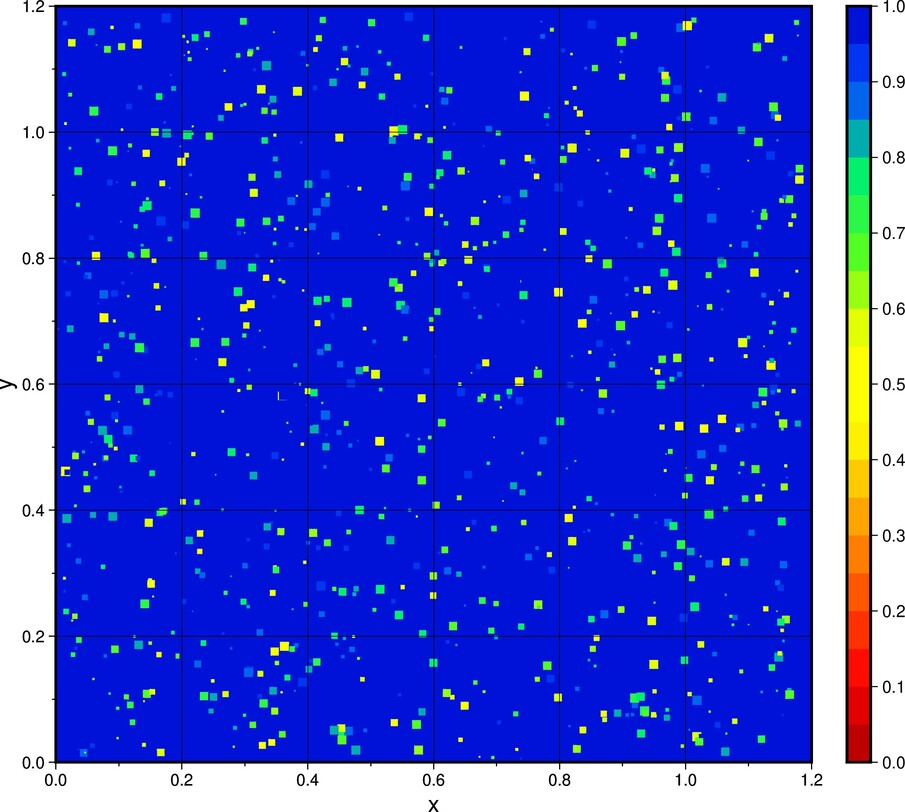
\includegraphics[width=5.2cm]{python_codes/fieldstone_171/images/uu000000.jpg}
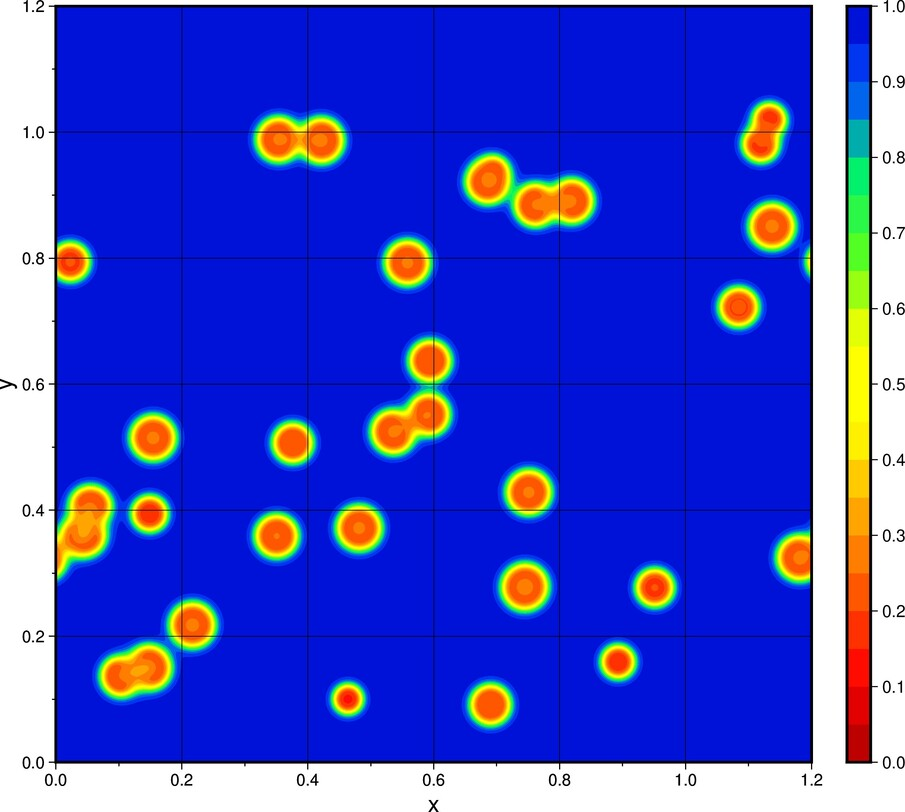
\includegraphics[width=5.2cm]{python_codes/fieldstone_171/images/uu000001.jpg}
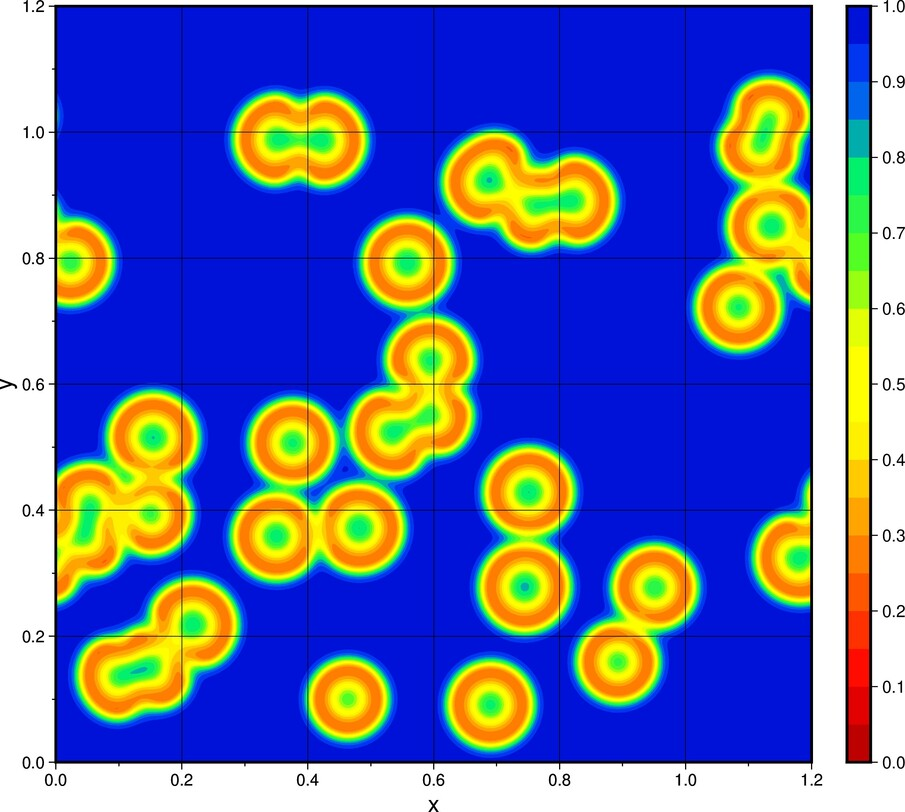
\includegraphics[width=5.2cm]{python_codes/fieldstone_171/images/uu000003.jpg}\\
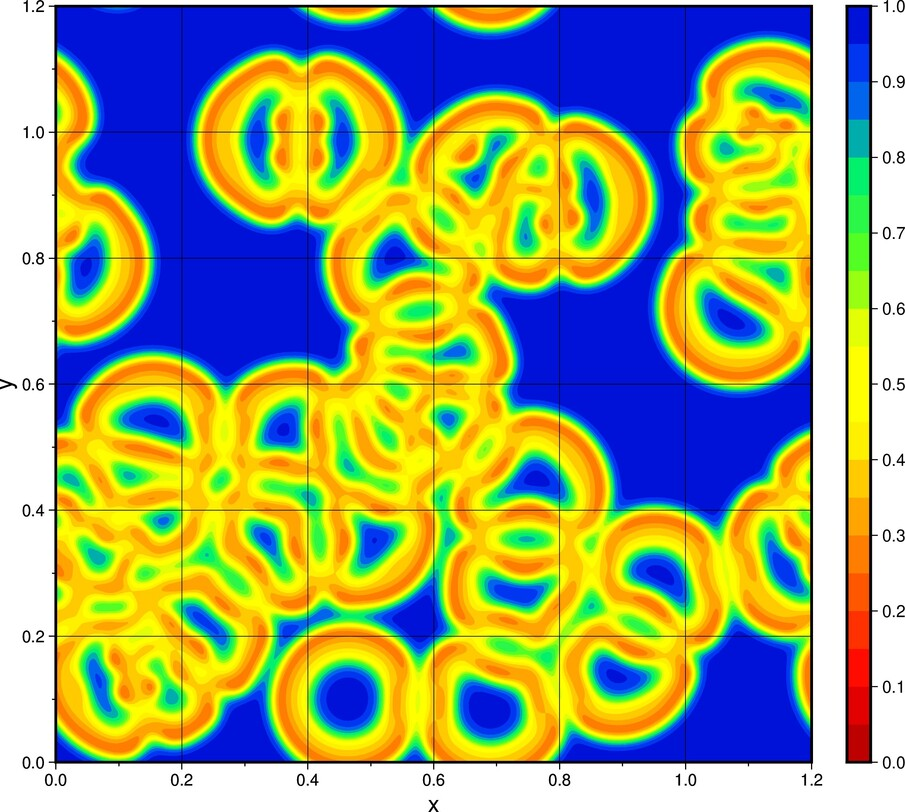
\includegraphics[width=5.2cm]{python_codes/fieldstone_171/images/uu000007.jpg}
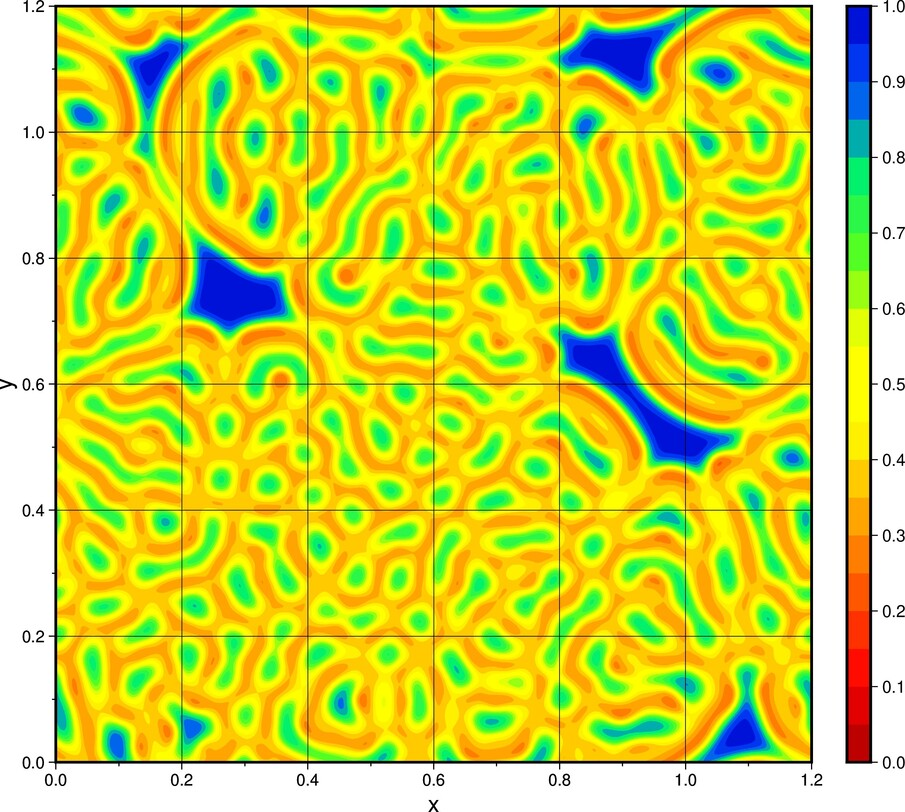
\includegraphics[width=5.2cm]{python_codes/fieldstone_171/images/uu000012.jpg}
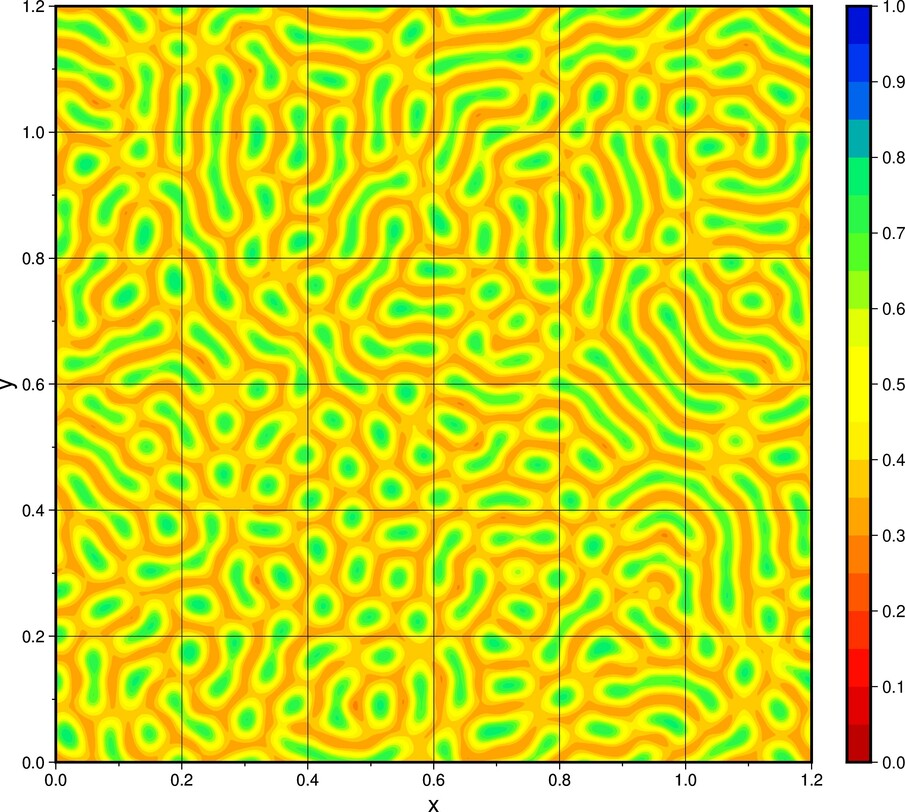
\includegraphics[width=5.2cm]{python_codes/fieldstone_171/images/uu000020.jpg}\\
{\captionfont Solved in on a GPU, which did this in about a day, on 4800x4800.}
\end{center}

%%%%%%%%%%%%%%%%%%%%%%%%%%%%%%%%%%%%%%%%%%%%%%%%%%%%%%%%%%%%%%%%%%%%%%%%%%%
\section*{Classification}

The topic of classification is important here since each greek letter
should correspond to a unique dynamical evolution/pattern
Unfortunately, while every paper published after 1993 quotes Pearson and 
his 12 models, the Pearson paper itself is rather ambiguous about 
the exact $F,k$ values for each of the 12 models shown in its Fig. 2.

The classification is then as follows:
\begin{center}
\begin{tabular}{lllll}
&Munafo & Munafo & Gandy \& Nelson 2022 & Har-Shemesh et al 2016 \\ 
\hline
alpha   & $F=0.010,k=0.047$  &$F=0.014,k=0.053$ & $F=0.010,k=0.050$ & $F=0.0175,k=0.0504$ \\
beta    & $F=0.014,k=0.039$  &$F=0.026,k=0.051$ &                   & \\
gamma   & $F=0.022,k=0.051$  &$F=0.026,k=0.055$ & $F=0.025,k=0.054$ & \\
delta   & $F=0.030,k=0.055$  &$F=0.042,k=0.059$ & $F=0.025,k=0.052$ & \\
epsilon & $F=0.018,k=0.055$  &$F=0.022,k=0.059$ &                   & $F=0.0208,k=0.0576$\\
zeta    & $F=0.022,k=0.061$  &$F=0.026,k=0.059$ &                   & \\
eta     & $F=0.034,k=0.063$  &	                &                   & $F=0.0404,k=0.0638$ \\
theta   & $F=0.030,k=0.057$  &$F=0.038,k=0.061$ &                   & $F=0.0295,k=0.0561$\\
iota    & $F=0.046,k=0.0594$ &                  &                   & \\
kappa   & $F=0.050,k=0.063$  &$F=0.058,k=0.063$ &                   & \\
lambda  & $F=0.026,k=0.061$  &$F=0.034,k=0.065$ &                   & $F=0.0392,k=0.0649$ \\
mu      & $F=0.046,k=0.065$  &$F=0.058,k=0.065$ & $F=0.050,k=0.064$ & $F=0.0416,k=0.0625$ \\
nu      & $F=0.054,k=0.067$  &$F=0.082,k=0.063$ &                   & \\
xi      & $F=0.010,k=0.041$  &$F=0.014,k=0.047$ & $F=0.010,k=0.042$ & \\
pi      & $F=0.062,k=0.061$  &                  &                   & \\
rho     & $F=0.090,k=0.059$  &$F=0.102,k=0.055$ &                   & \\
sigma   & $F=0.090,k=0.057$  &$F=0.110,k=0.0523$& $F=0.095,k=0.056$ & \\
\hline
\end{tabular}
\end{center}


%%%%%%%%%%%%%%%%%%%%%%%%%%%%%%%%%%%%%%%%%%%%%%%%%%%%%%%%%%%%%%%%%%%%%%%%%%%%%%%%%%%%%
\section*{About the methods of this \stone}

The domain is a cuboid of size $L_x \times L_y \times L_z$ in 3d and 
a square of size $L_x \times L_z$ is 2d.
It is discretised by means of a $nnx \times nny \times nnz = NP$ grid
in 3d and a $nnx \times nnz = NP$ grid in 2d.
The default here is $L_x=L_z=2.5$.

We are dealing with a set of coupled nonlinear PDEs to which there is no analytical solution.
We must then solve them by means of a numerical method. 
A Finite Difference (FD) of Finite Element (FE) approach could of course be envisaged. 
The main difficulty then would be (as discussed in \stone~130) how to deal with the 
nonlinear terms. Also, based on 
the results presented above by Lukas and the literature 
it appears that a high resolution is necessary in order
to capture the features of certain models, i.e. of (at least?) $256\times 256$ nodes. 
This would yield {\it very} large linear systems to be solved hundreds/thousands of time.
Keeping this in mind we therefore decide to resort to the method of lines as in \stone~157,
i.e. an explicit Forward in Time scheme.

We discretise the Laplace operators as follows in 3d:
\[
\vec\nabla^2 u \simeq 
\frac{u_{i-1,j,k}-2u_{i,j,k}+u_{i+1,j,k}}{h_x^2} + 
\frac{u_{i,j-1,k}-2u_{i,j,k}+u_{i,j+1,k}}{h_y^2} + 
\frac{u_{i,j,k-1}-2u_{i,j,k}+u_{i,j,k+1}}{h_z^2} 
\]
and
\[
\vec\nabla^2 u \simeq 
\frac{u_{i-1,k}-2u_{i,k}+u_{i+1,k}}{h_x^2} + 
\frac{u_{i,k-1}-2u_{i,k}+u_{i,k+1}}{h_z^2} 
\]
in 2d, so that the PDEs can be discretised in space at a node $i$ as follows:
\begin{eqnarray}
\frac{\partial u_{i,j,k}}{\partial t} 
&=& D_u 
\left(
\frac{u_{i-1,j,k}-2u_{i,j,k}+u_{i+1,j,k}}{h_x^2} + 
\frac{u_{i,j-1,k}-2u_{i,j,k}+u_{i,j+1,k}}{h_y^2} + 
\frac{u_{i,j,k-1}-2u_{i,j,k}+u_{i,j,k+1}}{h_z^2} 
\right) \nn\\
&&- u_{i,j,k}v_{i,j,k}^2 + F(1-u_{i,j,k}) 
\nn\\
\frac{\partial v_{i,j,k}}{\partial t} &=& D_v 
\left(
\frac{v_{i-1,j,k}-2v_{i,j,k}+v_{i+1,j,k}}{h_x^2} + 
\frac{v_{i-1,j,k}-2v_{i,j,k}+v_{i+1,j,k}}{h_y^2} + 
\frac{v_{i,j,k-1}-2v_{i,j,k}+v_{i,j,k+1}}{h_z^2} 
\right) \nn\\
&&
+ u_{i,j,k}v_{i,j,k}^2 - (F+k)v_{i,j,k}
\end{eqnarray}
In two dimensions these equations become simply:

\begin{eqnarray}
\frac{\partial u_{i,k}}{\partial t} 
&=& D_u 
\left(
\frac{u_{i-1,k}-2u_{i,k}+u_{i+1,k}}{h_x^2} + 
\frac{u_{i,k-1}-2u_{i,k}+u_{i,k+1}}{h_z^2} 
\right)
- u_{i,k}v_{i,k}^2 + F(1-u_{i,k}) 
\nn\\
\frac{\partial v_{i,k}}{\partial t} &=& D_v 
\left(
\frac{v_{i-1,k}-2v_{i,k}+v_{i+1,k}}{h_x^2} + 
\frac{v_{i,k-1}-2v_{i,k}+v_{i,k+1}}{h_z^2} 
\right) 
+ u_{i,k}v_{i,k}^2 - (F+k)v_{i,k}
\end{eqnarray}

We then define $\vec{X}$ that is such that 
\[
\vec{X} = 
\left(
\begin{array}{c}
\vec{U} \\ \vec{V}
\end{array}
\right)
\] 
where $\vec{U}$ is the vector of all nodal $u$ values and 
$\vec{V}$ is the vector of all nodal $v$ values.

The equations above can then be written 
\[
\frac{d\vec{X}}{dt} 
= \vec{\cal F} (\vec{X})
\]
The right-hand side of this equation is then implemented as follows:
\begin{lstlisting}

def F_3d(Du,Dv,F,K,NP,hx,hy,hz,X):
    dX_dt=np.zeros(2*NP,dtype=np.float64)
    u=X[0:NP]
    v=X[NP:2*NP]
    ...
    counter=0
    for i in range(0,nnx):
        for j in range(0,nny):
            for k in range(0,nnz):
                ... 
                dX_dt[counter]=Duhx2*(u[front]-2*u[counter]+u[back])\
                              +Duhy2*(u[left] -2*u[counter]+u[right])\
                              +Duhz2*(u[top]  -2*u[counter]+u[bottom])\
                              -u[counter]*v[counter]**2+F*(1-u[counter])
                dX_dt[counter+NP]=Dvhx2*(v[front]-2*v[counter]+v[back])\
                                 +Dvhy2*(v[left] -2*v[counter]+v[right])\
                                 +Dvhz2*(v[top]  -2*v[counter]+v[bottom])\
                                 +u[counter]*v[counter]**2-(F+K)*v[counter]
                counter+=1
    ...
    return dX_dt
\end{lstlisting}
Note that the code above is not complete and only serves as an 
illustration of the structure of the function.
There is of course a similar function for the 2d case.
Both \lstinline{F_2d} and \lstinline{F_3d} are jitted with
\lstinline{@numba.njit} and it makes them at least 100 times faster.

Periodic boundary conditions are implemented\footnote{This should be described}.

The solution vectors $\vec{U}$ and $\vec{V}$ are then exported to 
a vtu file every so often (controlled by the \lstinline{every_vtu} parameter),
and in 2d png files are automatically generated (controlled by 
the \lstinline{every_png} parameter).

A good starting point for the timestep is 0.1 dimensionless units, but 
(very) high resolutions may require much smaller values.
Note that the CFL condition number for diffusion is $\propto h^2/\kappa$, 
so that when resolution is halved the time step should probably be divided by four. 

There are three initial conditions, as controlled by the \lstinline{init} parameter.
Initial conditions are nearly always specified in the literature. For example, we
read in \cite{haqh16}: 
``The simulation was started with an initial condition of the
red state (u,v)=(1,0) with a finite perturbation in the form of a 20x20 square in the
center of the simulation grid in the state (u,v)=(0.5, 0.25) and an additional Gaussian
noise with an amplitude of 0.05 covering the entire simulation grid.''


\begin{itemize}
\item \lstinline{init=1}:
The initial condition is as follows: the field $u$ is initialized
to random values between 0.8 and 1 while the field $v$ is 
initialized to random values between 0 and 0.2:
\begin{lstlisting}
for i in range(0,NP):
    u[i]=random.uniform(0.8,1) # close to 1
    v[i]=random.uniform(0,0.2) # close to 0 
\end{lstlisting}
A number \lstinline{nseed} of square seeds is added on top
of these fields: their location is random and their field values too,
see 2d example:
\begin{lstlisting}
for iseed in range(nseed):
    xs=random.uniform(0+2*seed_size,Lx-2*seed_size)
    zs=random.uniform(0+2*seed_size,Lz-2*seed_size)
    for i in range(0,NP):
        if abs(x[i]-xs)<seed_size and\
           abs(z[i]-zs)<seed_size :
           u[i]=random.uniform(0.5,1)
    xs=random.uniform(0+2*seed_size,Lx-2*seed_size)
    zs=random.uniform(0+2*seed_size,Lz-2*seed_size)
    for i in range(0,NP):
        if abs(x[i]-xs)<seed_size and\
           abs(z[i]-zs)<seed_size :
           v[i]=random.uniform(0.,0.5)
\end{lstlisting}

\item \lstinline{init=2}: 
This corresponds to the case where 3 discs (cylinders in 3d)
are implemented. There is no random component and it allows 
us to test the code in a deterministic fashion (see 
tests of RK methods later)
\begin{lstlisting}
for i in range(0,NP):
    if (x[i]-Lx/3)**2+(z[i]-Lz/3)**2<0.2:
       u[i]=1
       v[i]=0.5
    if (x[i]-Lx*0.67)**2+(z[i]-Lz/2)**2<0.2:
       u[i]=0.5
       v[i]=0.25
    if (x[i]-Lx*0.5)**2+(z[i]-Lz*0.75)**2<0.08:
       u[i]=0.7
       v[i]=0.125
\end{lstlisting}

\item \lstinline{init=3}: 
This is the starting condition of \textcite{pear93} (1993).
\begin{lstlisting}
   u[:]=1
   v[:]=0
   for i in range(0,NP):
       if abs(x[i]-Lx/2)<0.2 and abs(z[i]-Lz/2)<0.2:
          u[i]=1/2+random.uniform(-0.01,0.01)
          v[i]=1/4+random.uniform(-0.01,0.01)
\end{lstlisting}

\item \lstinline{init=4}: I found it 
online\footnote{\url{https://github.com/cselab/gray-scott/blob/master/python/gray_scott.py}}
but it was written for a simulation taking place in a $[-1:1]\times[-1:1]$ domain.
I then displace the gaussians so as to bring them to the middle of our domain.

\begin{lstlisting}
for i in range(0,NP):
    xi=x[i]-Lx/2
    zi=z[i]-Lz/2
    u[i]=1-np.exp(-80*((xi+0.05)**2+(zi+0.05)**2))
    v[i]=np.exp(-80*((xi-0.05)**2+(zi-0.05)**2))
\end{lstlisting}

This initial condition is simple, seems to work with all greek letter models, and is 
deterministic (no randomness) so that it lends itself to testing (RK order, resolution, time step value, ...)

\end{itemize}



%--------------------------------------------------------
\subsubsection*{Time-stepping}


The code implements a large family of Runge-Kutta algorithms, all described in 
Section~\ref{MMM-ss:rkm}.
In what follows we assume that a time step $\delta t$ has been chosen. 
(embedded methods should probably be considered in the future).

\begin{itemize}

%--------------------------------------
\item 1st-order RK (\lstinline{scheme='RK1'})
Starting from the ODE above we can write
\[
\frac{\vec{X}^{n+1} -\vec{X}^{n} }{\delta t} = \vec{\cal F} (\vec{X}^n)
\]
or, 
\[
\vec{X}^{n+1}
=
\vec{X}^{n} + \vec{\cal F} (\vec{X}^n) \delta t
\]
which translates into
\begin{lstlisting}
for istep in range(0,nstep+1):
    X[:]+=F_2d(Du,Dv,Feed,Kill,NP,hx,hz,X)*dt
\end{lstlisting}

%--------------------------------------
\item 2nd-order RK (\lstinline{scheme='RK2'})
\begin{lstlisting}
for istep in range(0,nstep+1):
    k1=F_2d(Du,Dv,Feed,Kill,NP,hx,hz,X     )*dt
    k2=F_2d(Du,Dv,Feed,Kill,NP,hx,hz,X+k1/2)*dt
    X[:]+=k2
\end{lstlisting}

%--------------------------------------
\item 2nd-order RK (\lstinline{scheme='Heun'})

\begin{lstlisting}
for istep in range(0,nstep+1):
    k1=F_2d(Du,Dv,Feed,Kill,NP,hx,hz,X   )*dt
    k2=F_2d(Du,Dv,Feed,Kill,NP,hx,hz,X+k1)*dt
    X[:]+=(k1+k2)/2
\end{lstlisting}

%--------------------------------------
\item 3rd-order RK (\lstinline{scheme='RK3'})

\begin{eqnarray}
\vec{k}_1 &=& \vec{\cal F}(\vec{X}_n) \cdot \delta t\nn\\
\vec{k}_2 &=& \vec{\cal F}(\vec{X}_n+ \frac{1}{2} \vec{k}_1) \cdot \delta t \nn\\
\vec{k}_3 &=& \vec{\cal F}(\vec{X}_n -\vec{k}_1 +2\vec{k}_2) \cdot \delta t \nn\\
\vec{X}_{n+1} &=& \vec{X}_n + \frac{1}{6}\left(\vec{k}_1 + 4\vec{k}_2 + \vec{k}_3 \right)
\end{eqnarray}

\begin{lstlisting}
for istep in range(0,nstep+1):
    k1=F_2d(Du,Dv,Feed,Kill,NP,hx,hz,X        )*dt
    k2=F_2d(Du,Dv,Feed,Kill,NP,hx,hz,X+k1/2   )*dt
    k3=F_2d(Du,Dv,Feed,Kill,NP,hx,hz,X-k1+2*k2)*dt
    X[:]+=(k1+4*k2+k3)/6
\end{lstlisting}


%--------------------------------------
\item 4th-order RK\footnote{\url{https://en.wikipedia.org/wiki/Runge-Kutta_methods}}
(\lstinline{scheme='RK4'})

\begin{eqnarray}
\vec{k}_1 &=& \vec{\cal F}(\vec{X}_n) \cdot \delta t\nn\\
\vec{k}_2 &=& \vec{\cal F}(\vec{X}_n+ \frac12\vec{k}_1) \cdot \delta t \nn\\
\vec{k}_3 &=& \vec{\cal F}(\vec{X}_n+ \frac12\vec{k}_2) \cdot \delta t \nn\\
\vec{k}_4 &=& \vec{\cal F}(\vec{X}_n+ \vec{k}_3)    \cdot \delta t \nn \\
\vec{X}_{n+1} &=& \vec{X}_n + \frac{1}{6}\left(\vec{k}_1 + 2\vec{k}_2 + 2\vec{k}_3 + \vec{k}_4\right)
\end{eqnarray}

This translates very simply as follows into code:
\begin{lstlisting}
for istep in range(0,nstep+1):
    k1=F_2d(Du,Dv,Feed,Kill,NP,hx,hz,X     )*dt
    k2=F_2d(Du,Dv,Feed,Kill,NP,hx,hz,X+k1/2)*dt
    k3=F_2d(Du,Dv,Feed,Kill,NP,hx,hz,X+k2/2)*dt
    k4=F_2d(Du,Dv,Feed,Kill,NP,hx,hz,X+k3  )*dt
    X[:]+=(k1+2*k2+2*k3+k4)/6
\end{lstlisting}


%--------------------------------------
\item 4th-order RK (\lstinline{scheme='RK38'})

\begin{lstlisting}
for istep in range(0,nstep+1):
    k1=F_2d(Du,Dv,Feed,Kill,NP,hx,hz,X         )*dt
    k2=F_2d(Du,Dv,Feed,Kill,NP,hx,hz,X+k1/3    )*dt
    k3=F_2d(Du,Dv,Feed,Kill,NP,hx,hz,X-k1/3+k2 )*dt
    k4=F_2d(Du,Dv,Feed,Kill,NP,hx,hz,X+k1-k2+k3)*dt
    X[:]+=(k1+3*k2+3*k3+k4)/8
\end{lstlisting}

%--------------------------------------
\item 5th-order RK (\lstinline{scheme='RK5'})

\begin{lstlisting}
for istep in range(0,nstep+1):
    k1=F_2d(Du,Dv,Feed,Kill,NP,hx,hz,X                                    )*dt
    k2=F_2d(Du,Dv,Feed,Kill,NP,hx,hz,X+k1/3                               )*dt
    k3=F_2d(Du,Dv,Feed,Kill,NP,hx,hz,X+k1*4/25+k2*6/25                    )*dt
    k4=F_2d(Du,Dv,Feed,Kill,NP,hx,hz,X+k1/4   -k2*3    +k3*15/4           )*dt
    k5=F_2d(Du,Dv,Feed,Kill,NP,hx,hz,X+k1*2/27+k2*10/9 -k3*50/81 +k4*8/81 )*dt
    k6=F_2d(Du,Dv,Feed,Kill,NP,hx,hz,X+k1*2/25+k2*12/25+k3*2/15  +k4*8/75 )*dt
    X[:]+=(k1*23+125*k3-81*k5+125*k6)/192
\end{lstlisting}

%--------------------------------------
\item Runge-Kutta-Fehlberg\footnote{\url{https://ketch.github.io/numipedia/methods/Fehlberg45.html}} 
(\lstinline{scheme='RKF'})

The coefficients are obtained from the following Butcher tableau.

\begin{align} 
\begin{array}{c|cccccc} 
& & & & & & \\ 
\frac{1}{4} & \frac{1}{4} & & & & & \\ 
\frac{3}{8} & \frac{3}{32} & \frac{9}{32} & & & & \\ 
\frac{12}{13} & \frac{1932}{2197} & - \frac{7200}{2197} & \frac{7296}{2197} & & & \\ 
1 & \frac{439}{216} & -8 & \frac{3680}{513} & - \frac{845}{4104} & & \\ 
\frac{1}{2} & - \frac{8}{27} & 2 & - \frac{3544}{2565} & \frac{1859}{4104} & - \frac{11}{40} & \\ 
\hline & \frac{16}{135} & & \frac{6656}{12825} & \frac{28561}{56430} & - \frac{9}{50} & \frac{2}{55}\\ 
& \frac{25}{216} & & \frac{1408}{2565} & \frac{2197}{4104} & - \frac{1}{5} & 
\end{array}
\end{align}


\end{itemize}

TODO:

try implicit ? if I only keep the Laplace terms in the matrix the matrix does not change, only the rhs.

add colorbar to png plots

change/prescribe colorscale python

use python function to integrate ? a la rhymtite ? see stone 157

run 3D model(s). Which one ? why ?

extend code to 1D. apparently there is a fair bit of published work in 1d too.

Look at blob detection algorithms (haqh16) 

\newpage
%%%%%%%%%%%%%%%%%%%%%%%%%%%%%%%%%%%%%%%%%%%%%%%%%%%%%%%%%%%%%%%%%%%%%%%%%%%%%%%%%%%%%
\section*{Testing/benchmarking of R-K methods}

In this case we start with non random initial conditions (\lstinline{init=2}).
We run the zeta model and we find that it relaxes to the trivial solution $(u=1,v=0)$.
We use the {\tt script\_RKtest1} bash script.

\begin{center}
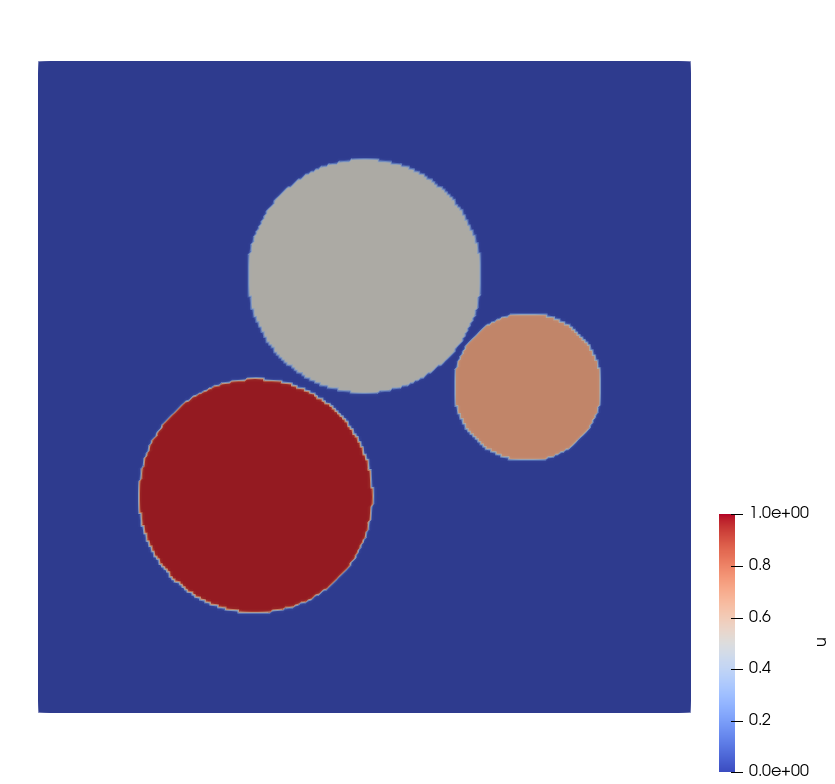
\includegraphics[height=6cm]{python_codes/fieldstone_171/RKtest1/u0}
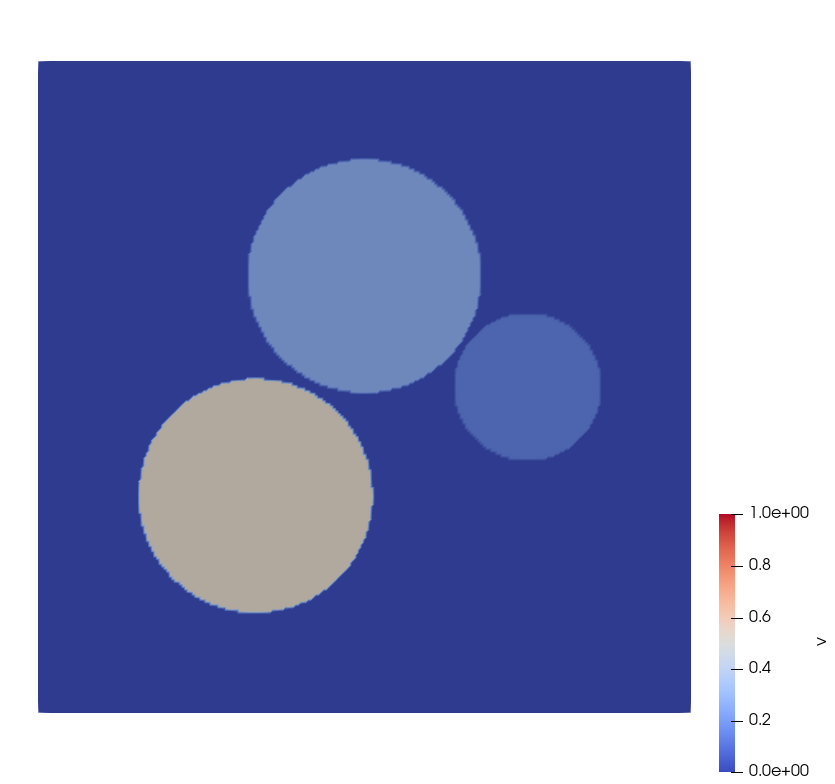
\includegraphics[height=6cm]{python_codes/fieldstone_171/RKtest1/v0}\\
{\captionfont $u$ and $v$ fields at $t=0$, resolution $257^2$.}
\end{center}

\begin{center}
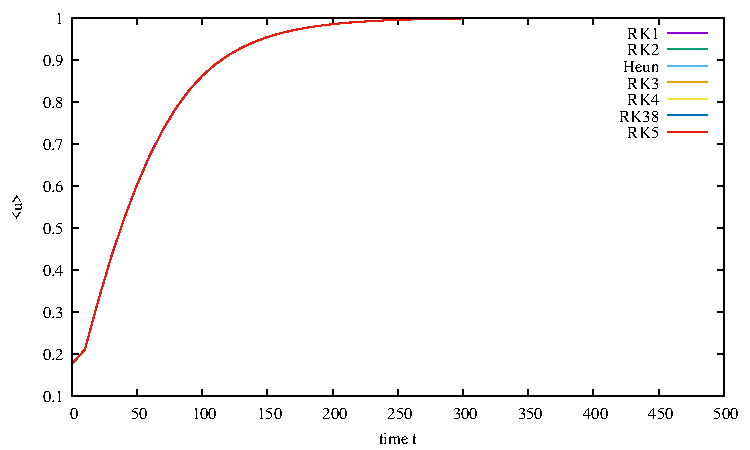
\includegraphics[width=8cm]{python_codes/fieldstone_171/RKtest1/avrg_u.pdf}
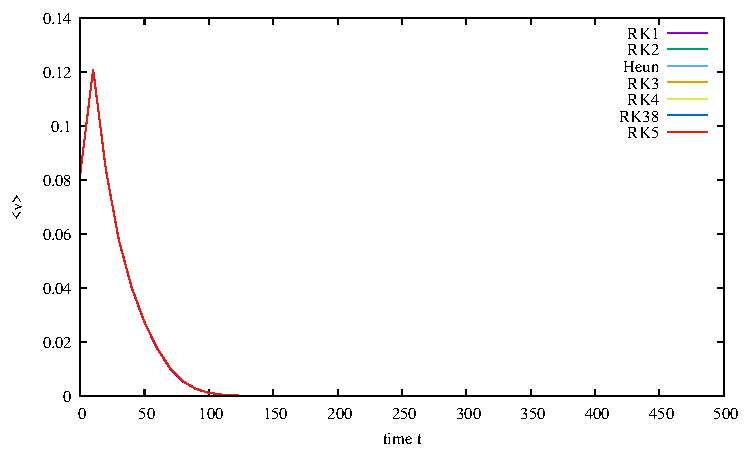
\includegraphics[width=8cm]{python_codes/fieldstone_171/RKtest1/avrg_v.pdf}\\
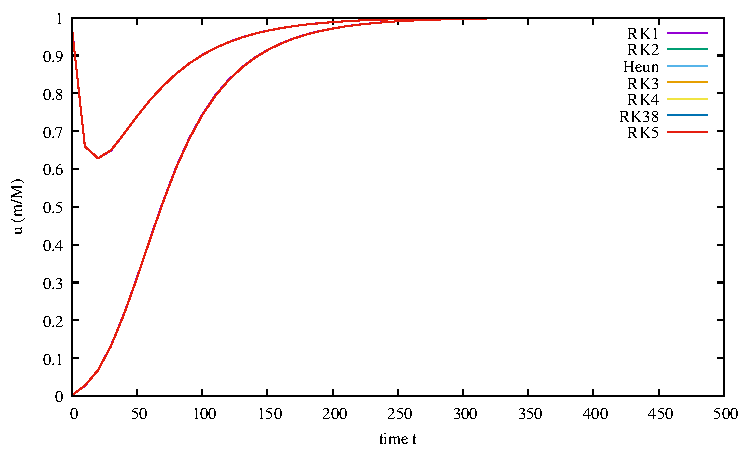
\includegraphics[width=8cm]{python_codes/fieldstone_171/RKtest1/stats_u.pdf}
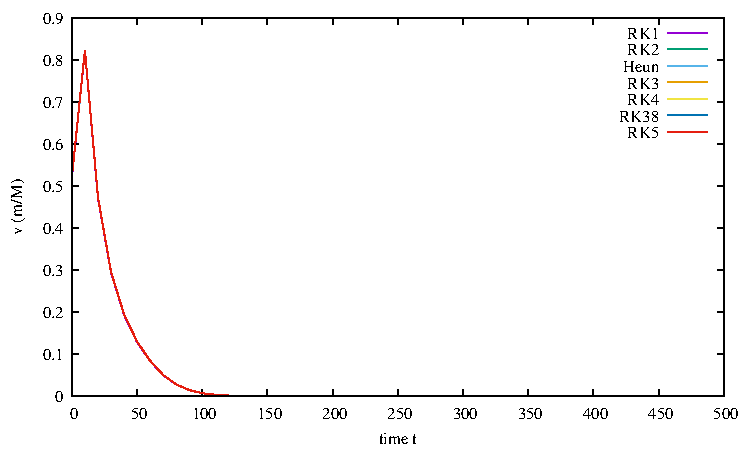
\includegraphics[width=8cm]{python_codes/fieldstone_171/RKtest1/stats_v.pdf}\\
{\captionfont Evolution of the averages and min/max values of fields $u$
and $v$ for all the RK methods, parameters of the zeta model.}
\end{center}

This is of course not a benchmark {\it per se}, but rather a sanity check that 
all RK methods yield the same results (down to a small difference).


\newpage
%%%%%%%%%%%%%%%%%%%%%%%%%%%%%%%%%%%%%%%%%%%%%%%%%%%%%%%%%%%%%%%%%%%%%%%%%%%%%%%%%%%%%
\section*{Testing/benchmarking of R-K methods (2)}

In this case we start with non random initial conditions (\lstinline{init=4}).
We run the alpha1 model. Resolution 257x257, dt=0.1, nstep=10,000.
We use the {\tt script\_RKtest2} bash script.

\begin{center}
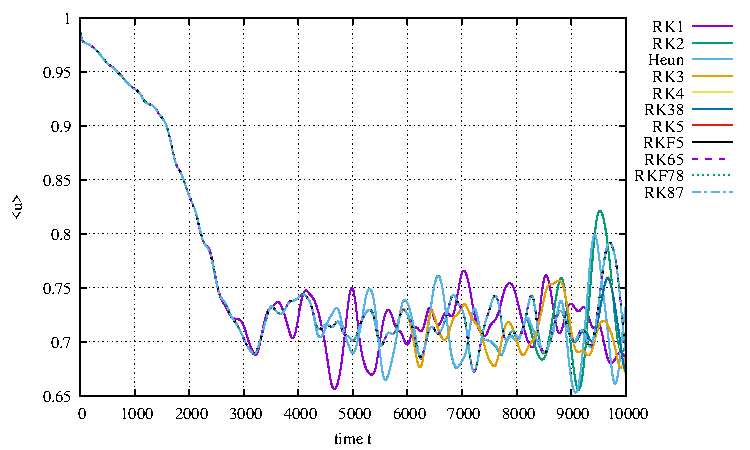
\includegraphics[width=8cm]{python_codes/fieldstone_171/RKtest2/avrg_u.pdf}
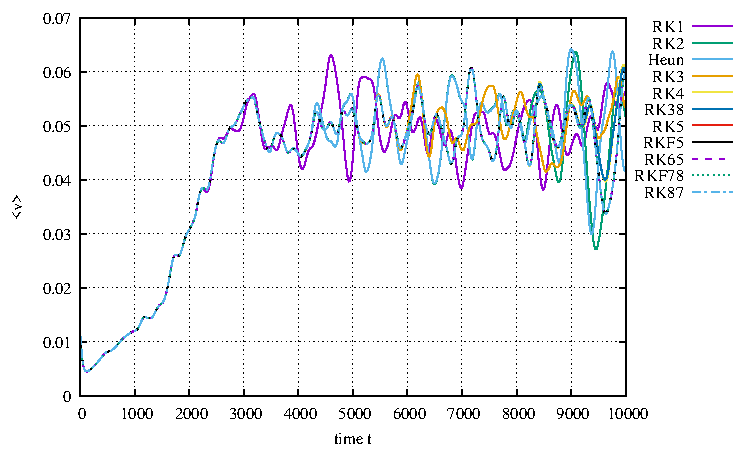
\includegraphics[width=8cm]{python_codes/fieldstone_171/RKtest2/avrg_v.pdf}\\
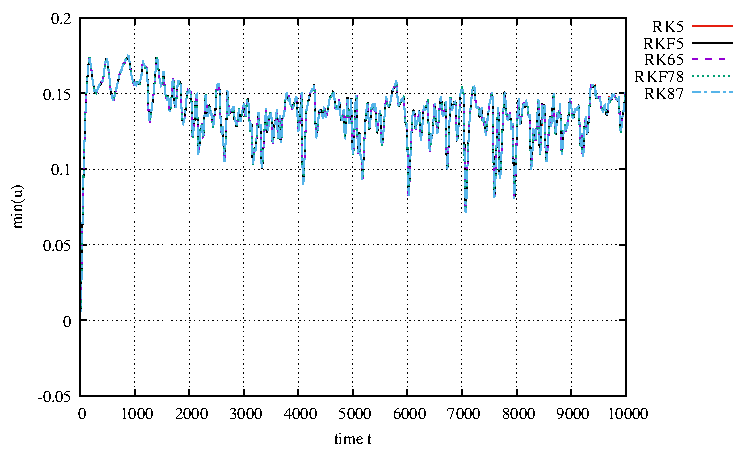
\includegraphics[width=8cm]{python_codes/fieldstone_171/RKtest2/stats_u.pdf}
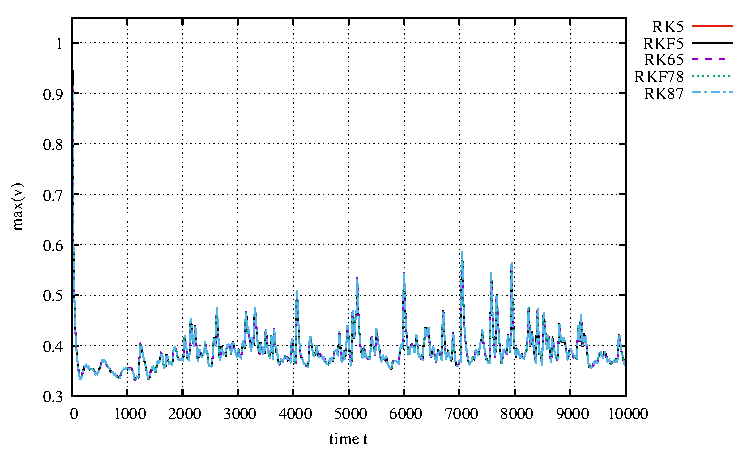
\includegraphics[width=8cm]{python_codes/fieldstone_171/RKtest2/stats_v.pdf}\\
{\captionfont Evolution of the averages and min/max values of fields $u$
and $v$ for all the RK methods, parameters of the alpha1 model.}
\end{center}

\begin{center}
\includegraphics[height=6cm]{python_codes/fieldstone_171/RKtest2/alpha1_solution_final_u_RKF.png}
\includegraphics[height=6cm]{python_codes/fieldstone_171/RKtest2/alpha1_solution_final_v_RKF.png}\\
{\captionfont $u$ and $v$ fields at the end of the run, resolution $257^2$.}
\end{center}


\newpage
%%%%%%%%%%%%%%%%%%%%%%%%%%%%%%%%%%%%%%%%%%%%%%%%%%%%%%%%%%%%%%%%%%%%%
\section*{Results: replicating the Pearson (1993) study (no random)}

The parameters of the paper are as follows: $D_u=2\cdot 10^{-5}$, $D_v=1\cdot 10^{-5}$,
$L_x=L_y=2.5$. FTCS scheme with Forward Euler, $\delta t=1$, 
resolution is $256 \times 256$.
Initially, the entire system was placed in
the trivial state (U = 1,V = 0). The 20 by 20 mesh point area located symmetrically
about the center of the grid was then
perturbed to ($U = 1/2,V = 1/4$). These
conditions were then perturbed with $\pm 1\%$
random noise in order to break the square
symmetry. The system was then integrated for 200,000 time steps.

The only difference with respect to the paper is that I resort to RK2.

The major issue here is that I cannot reproduce Fig 2 of the paper since the 
author does not provide the $(F,k)$ values for the 12 models. 
I then instead keep the nomenclature of Munafo for the 17 models
\footnote{In what follows the left column of the table is used to define the 17 
models} but we see that this is not necessarily reassuring since Munafo's letters 
do not always coincide with Pearson's:
\begin{center}
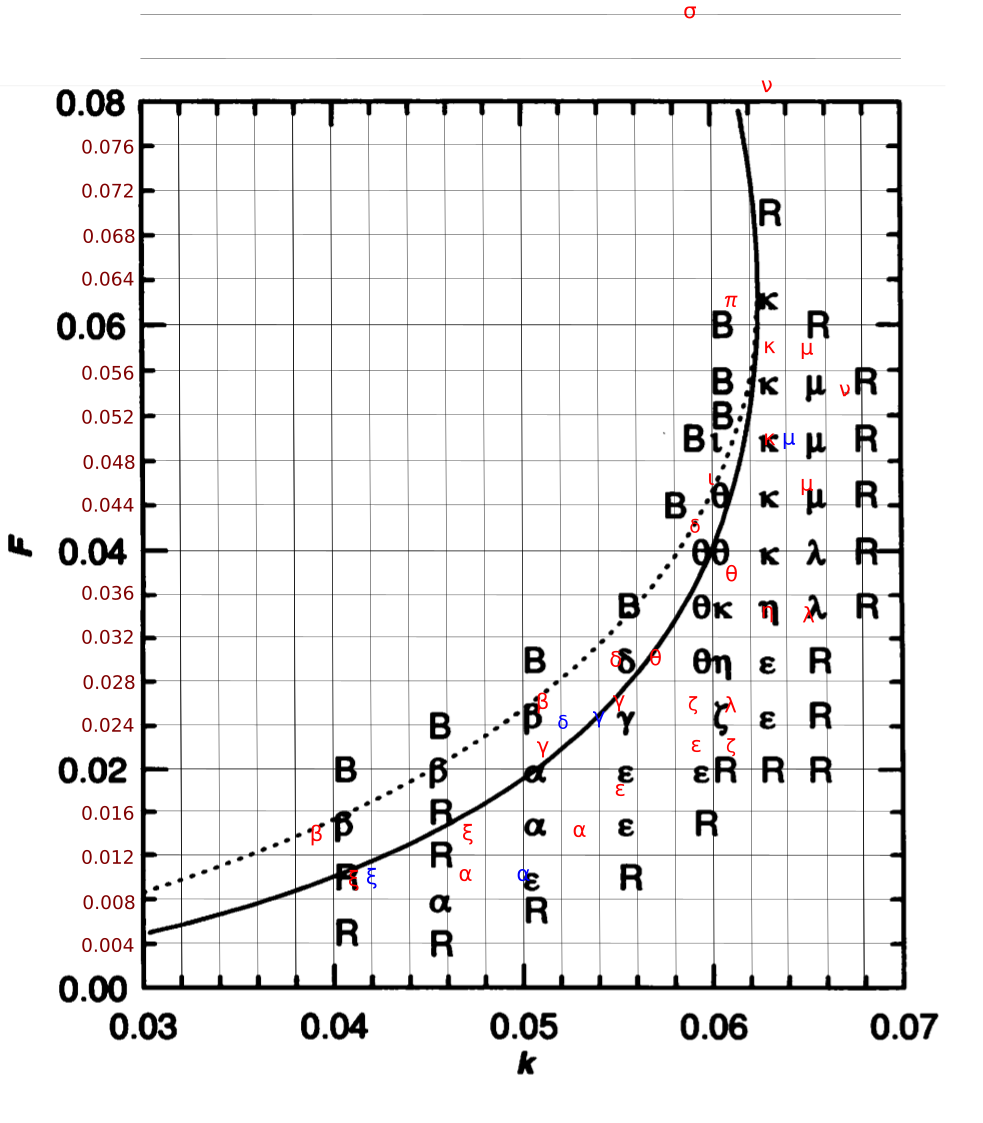
\includegraphics[height=14cm]{python_codes/fieldstone_171/images/drawing.png}\\
{\captionfont Fig 2 of Pearson. Red letters are Munafo's ones. 
Blue letters are from \cite{gane22}.}
\end{center}




All models start from the following initial condition ({\it the randomness was taken away}):
\begin{center}
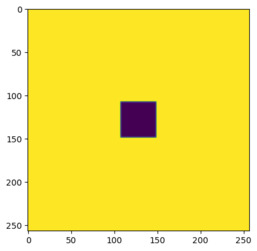
\includegraphics[width=4cm]{python_codes/fieldstone_171/pearson93/alpha_solution_0000000_u.png}
\end{center}

In what follows I only show the $u$ field for convenience.
Only 100,000 time steps are carried out.

\begin{itemize}
\item {\tt alpha} (in Pearson 1993)\\
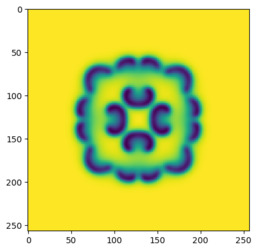
\includegraphics[width=1.4cm]{python_codes/fieldstone_171/pearson93/alpha_solution_0001000_u.png}
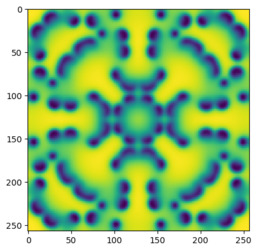
\includegraphics[width=1.4cm]{python_codes/fieldstone_171/pearson93/alpha_solution_0005000_u.png}
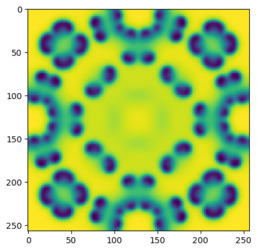
\includegraphics[width=1.4cm]{python_codes/fieldstone_171/pearson93/alpha_solution_0010000_u.png}
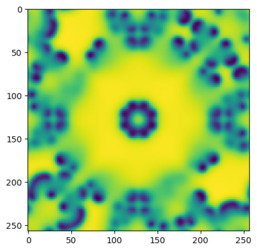
\includegraphics[width=1.4cm]{python_codes/fieldstone_171/pearson93/alpha_solution_0015000_u.png}
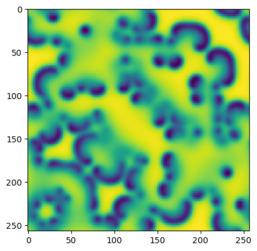
\includegraphics[width=1.4cm]{python_codes/fieldstone_171/pearson93/alpha_solution_0020000_u.png}
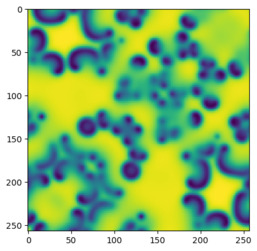
\includegraphics[width=1.4cm]{python_codes/fieldstone_171/pearson93/alpha_solution_0030000_u.png}
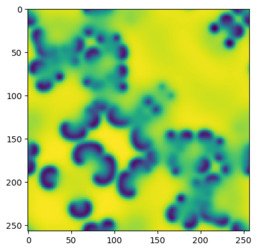
\includegraphics[width=1.4cm]{python_codes/fieldstone_171/pearson93/alpha_solution_0040000_u.png}
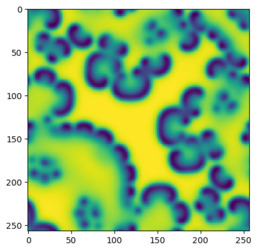
\includegraphics[width=1.4cm]{python_codes/fieldstone_171/pearson93/alpha_solution_0050000_u.png}
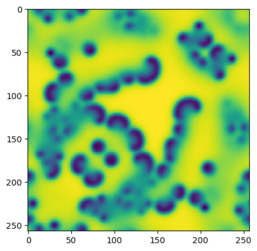
\includegraphics[width=1.4cm]{python_codes/fieldstone_171/pearson93/alpha_solution_0075000_u.png}
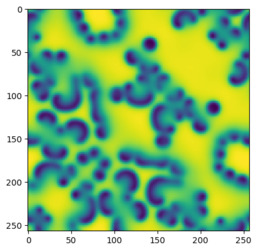
\includegraphics[width=1.4cm]{python_codes/fieldstone_171/pearson93/alpha_solution_final_u.png}
\item {\tt beta} (in Pearson 1993)\\
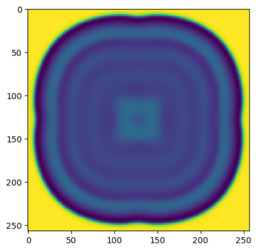
\includegraphics[width=1.4cm]{python_codes/fieldstone_171/pearson93/beta_solution_0001000_u.png}
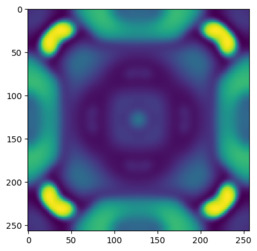
\includegraphics[width=1.4cm]{python_codes/fieldstone_171/pearson93/beta_solution_0005000_u.png}
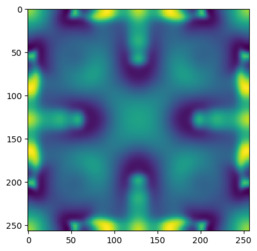
\includegraphics[width=1.4cm]{python_codes/fieldstone_171/pearson93/beta_solution_0010000_u.png}
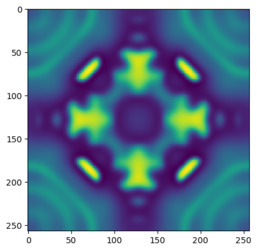
\includegraphics[width=1.4cm]{python_codes/fieldstone_171/pearson93/beta_solution_0015000_u.png}
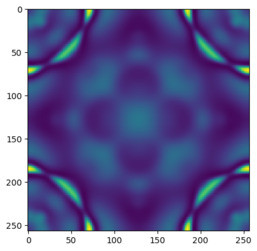
\includegraphics[width=1.4cm]{python_codes/fieldstone_171/pearson93/beta_solution_0020000_u.png}
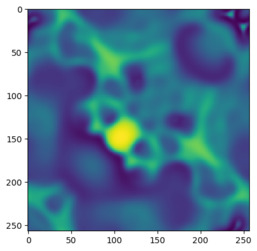
\includegraphics[width=1.4cm]{python_codes/fieldstone_171/pearson93/beta_solution_0030000_u.png}
\includegraphics[width=1.4cm]{python_codes/fieldstone_171/pearson93/beta_solution_0040000_u.png}
\includegraphics[width=1.4cm]{python_codes/fieldstone_171/pearson93/beta_solution_0050000_u.png}
\includegraphics[width=1.4cm]{python_codes/fieldstone_171/pearson93/beta_solution_0075000_u.png}
\includegraphics[width=1.4cm]{python_codes/fieldstone_171/pearson93/beta_solution_final_u.png}

\item {\tt gamma} (in Pearson 1993)\\
\includegraphics[width=1.4cm]{python_codes/fieldstone_171/pearson93/gamma_solution_0001000_u.png}
\includegraphics[width=1.4cm]{python_codes/fieldstone_171/pearson93/gamma_solution_0005000_u.png}
\includegraphics[width=1.4cm]{python_codes/fieldstone_171/pearson93/gamma_solution_0010000_u.png}
\includegraphics[width=1.4cm]{python_codes/fieldstone_171/pearson93/gamma_solution_0015000_u.png}
\includegraphics[width=1.4cm]{python_codes/fieldstone_171/pearson93/gamma_solution_0020000_u.png}
\includegraphics[width=1.4cm]{python_codes/fieldstone_171/pearson93/gamma_solution_0030000_u.png}
\includegraphics[width=1.4cm]{python_codes/fieldstone_171/pearson93/gamma_solution_0040000_u.png}
\includegraphics[width=1.4cm]{python_codes/fieldstone_171/pearson93/gamma_solution_0050000_u.png}
\includegraphics[width=1.4cm]{python_codes/fieldstone_171/pearson93/gamma_solution_0075000_u.png}
\includegraphics[width=1.4cm]{python_codes/fieldstone_171/pearson93/gamma_solution_final_u.png}


\item {\tt delta} (in Pearson 1993)\\
\includegraphics[width=1.4cm]{python_codes/fieldstone_171/pearson93/delta_solution_0001000_u.png}
\includegraphics[width=1.4cm]{python_codes/fieldstone_171/pearson93/delta_solution_0005000_u.png}
\includegraphics[width=1.4cm]{python_codes/fieldstone_171/pearson93/delta_solution_0010000_u.png}
\includegraphics[width=1.4cm]{python_codes/fieldstone_171/pearson93/delta_solution_0015000_u.png}
\includegraphics[width=1.4cm]{python_codes/fieldstone_171/pearson93/delta_solution_0020000_u.png}
\includegraphics[width=1.4cm]{python_codes/fieldstone_171/pearson93/delta_solution_0030000_u.png}
\includegraphics[width=1.4cm]{python_codes/fieldstone_171/pearson93/delta_solution_0040000_u.png}
\includegraphics[width=1.4cm]{python_codes/fieldstone_171/pearson93/delta_solution_0050000_u.png}
\includegraphics[width=1.4cm]{python_codes/fieldstone_171/pearson93/delta_solution_0075000_u.png}
\includegraphics[width=1.4cm]{python_codes/fieldstone_171/pearson93/delta_solution_final_u.png}

\item {\tt epsilon} (in Pearson 1993)\\
\includegraphics[width=1.4cm]{python_codes/fieldstone_171/pearson93/epsilon_solution_0001000_u.png}
\includegraphics[width=1.4cm]{python_codes/fieldstone_171/pearson93/epsilon_solution_0005000_u.png}
\includegraphics[width=1.4cm]{python_codes/fieldstone_171/pearson93/epsilon_solution_0010000_u.png}
\includegraphics[width=1.4cm]{python_codes/fieldstone_171/pearson93/epsilon_solution_0015000_u.png}
\includegraphics[width=1.4cm]{python_codes/fieldstone_171/pearson93/epsilon_solution_0020000_u.png}
\includegraphics[width=1.4cm]{python_codes/fieldstone_171/pearson93/epsilon_solution_0030000_u.png}
\includegraphics[width=1.4cm]{python_codes/fieldstone_171/pearson93/epsilon_solution_0040000_u.png}
\includegraphics[width=1.4cm]{python_codes/fieldstone_171/pearson93/epsilon_solution_0050000_u.png}
\includegraphics[width=1.4cm]{python_codes/fieldstone_171/pearson93/epsilon_solution_0075000_u.png}
\includegraphics[width=1.4cm]{python_codes/fieldstone_171/pearson93/epsilon_solution_final_u.png}

\item {\tt zeta} (in Pearson 1993)\\
\includegraphics[width=1.4cm]{python_codes/fieldstone_171/pearson93/zeta_solution_0001000_u.png}
\includegraphics[width=1.4cm]{python_codes/fieldstone_171/pearson93/zeta_solution_0010000_u.png}
\includegraphics[width=1.4cm]{python_codes/fieldstone_171/pearson93/zeta_solution_0030000_u.png}
\includegraphics[width=1.4cm]{python_codes/fieldstone_171/pearson93/zeta_solution_0050000_u.png}
\includegraphics[width=1.4cm]{python_codes/fieldstone_171/pearson93/zeta_solution_final_u.png}


\item {\tt eta} (in Pearson 1993)\\
\includegraphics[width=1.4cm]{python_codes/fieldstone_171/pearson93/eta_solution_0001000_u.png}
\includegraphics[width=1.4cm]{python_codes/fieldstone_171/pearson93/eta_solution_0005000_u.png}
\includegraphics[width=1.4cm]{python_codes/fieldstone_171/pearson93/eta_solution_0010000_u.png}
\includegraphics[width=1.4cm]{python_codes/fieldstone_171/pearson93/eta_solution_0015000_u.png}
\includegraphics[width=1.4cm]{python_codes/fieldstone_171/pearson93/eta_solution_0020000_u.png}
\includegraphics[width=1.4cm]{python_codes/fieldstone_171/pearson93/eta_solution_0030000_u.png}
\includegraphics[width=1.4cm]{python_codes/fieldstone_171/pearson93/eta_solution_0040000_u.png}
\includegraphics[width=1.4cm]{python_codes/fieldstone_171/pearson93/eta_solution_0050000_u.png}
\includegraphics[width=1.4cm]{python_codes/fieldstone_171/pearson93/eta_solution_0075000_u.png}
\includegraphics[width=1.4cm]{python_codes/fieldstone_171/pearson93/eta_solution_final_u.png}

\item {\tt theta} (in Pearson 1993)\\
\includegraphics[width=1.4cm]{python_codes/fieldstone_171/pearson93/theta_solution_0001000_u.png}
\includegraphics[width=1.4cm]{python_codes/fieldstone_171/pearson93/theta_solution_0005000_u.png}
\includegraphics[width=1.4cm]{python_codes/fieldstone_171/pearson93/theta_solution_0010000_u.png}
\includegraphics[width=1.4cm]{python_codes/fieldstone_171/pearson93/theta_solution_0015000_u.png}
\includegraphics[width=1.4cm]{python_codes/fieldstone_171/pearson93/theta_solution_0020000_u.png}
\includegraphics[width=1.4cm]{python_codes/fieldstone_171/pearson93/theta_solution_0030000_u.png}
\includegraphics[width=1.4cm]{python_codes/fieldstone_171/pearson93/theta_solution_0040000_u.png}
\includegraphics[width=1.4cm]{python_codes/fieldstone_171/pearson93/theta_solution_0050000_u.png}
\includegraphics[width=1.4cm]{python_codes/fieldstone_171/pearson93/theta_solution_0075000_u.png}
\includegraphics[width=1.4cm]{python_codes/fieldstone_171/pearson93/theta_solution_final_u.png}









\item {\tt iota} (in Pearson 1993)\\
\includegraphics[width=1.4cm]{python_codes/fieldstone_171/pearson93/iota_solution_0001000_u.png}
\includegraphics[width=1.4cm]{python_codes/fieldstone_171/pearson93/iota_solution_0005000_u.png}
\includegraphics[width=1.4cm]{python_codes/fieldstone_171/pearson93/iota_solution_0010000_u.png}
\includegraphics[width=1.4cm]{python_codes/fieldstone_171/pearson93/iota_solution_0015000_u.png}
\includegraphics[width=1.4cm]{python_codes/fieldstone_171/pearson93/iota_solution_0020000_u.png}
\includegraphics[width=1.4cm]{python_codes/fieldstone_171/pearson93/iota_solution_0030000_u.png}
\includegraphics[width=1.4cm]{python_codes/fieldstone_171/pearson93/iota_solution_0040000_u.png}
\includegraphics[width=1.4cm]{python_codes/fieldstone_171/pearson93/iota_solution_0050000_u.png}
\includegraphics[width=1.4cm]{python_codes/fieldstone_171/pearson93/iota_solution_0075000_u.png}
\includegraphics[width=1.4cm]{python_codes/fieldstone_171/pearson93/iota_solution_final_u.png}
\item {\tt kappa} (in Pearson 1993)\\
\includegraphics[width=1.4cm]{python_codes/fieldstone_171/pearson93/kappa_solution_0001000_u.png}
\includegraphics[width=1.4cm]{python_codes/fieldstone_171/pearson93/kappa_solution_0005000_u.png}
\includegraphics[width=1.4cm]{python_codes/fieldstone_171/pearson93/kappa_solution_0010000_u.png}
\includegraphics[width=1.4cm]{python_codes/fieldstone_171/pearson93/kappa_solution_0015000_u.png}
\includegraphics[width=1.4cm]{python_codes/fieldstone_171/pearson93/kappa_solution_0020000_u.png}
\includegraphics[width=1.4cm]{python_codes/fieldstone_171/pearson93/kappa_solution_0030000_u.png}
\includegraphics[width=1.4cm]{python_codes/fieldstone_171/pearson93/kappa_solution_0040000_u.png}
\includegraphics[width=1.4cm]{python_codes/fieldstone_171/pearson93/kappa_solution_0050000_u.png}
\includegraphics[width=1.4cm]{python_codes/fieldstone_171/pearson93/kappa_solution_0075000_u.png}
\includegraphics[width=1.4cm]{python_codes/fieldstone_171/pearson93/kappa_solution_final_u.png}

\item {\tt lambda} (in Pearson 1993)\\
\includegraphics[width=1.4cm]{python_codes/fieldstone_171/pearson93/lambda_solution_0001000_u.png}
\includegraphics[width=1.4cm]{python_codes/fieldstone_171/pearson93/lambda_solution_0005000_u.png}
\includegraphics[width=1.4cm]{python_codes/fieldstone_171/pearson93/lambda_solution_0010000_u.png}
\includegraphics[width=1.4cm]{python_codes/fieldstone_171/pearson93/lambda_solution_0015000_u.png}
\includegraphics[width=1.4cm]{python_codes/fieldstone_171/pearson93/lambda_solution_0020000_u.png}
\includegraphics[width=1.4cm]{python_codes/fieldstone_171/pearson93/lambda_solution_0030000_u.png}
\includegraphics[width=1.4cm]{python_codes/fieldstone_171/pearson93/lambda_solution_0040000_u.png}
\includegraphics[width=1.4cm]{python_codes/fieldstone_171/pearson93/lambda_solution_0050000_u.png}
\includegraphics[width=1.4cm]{python_codes/fieldstone_171/pearson93/lambda_solution_0075000_u.png}
\includegraphics[width=1.4cm]{python_codes/fieldstone_171/pearson93/lambda_solution_final_u.png}

\item {\tt mu} (in Pearson 1993)\\
\includegraphics[width=1.4cm]{python_codes/fieldstone_171/pearson93/mu_solution_0001000_u.png}
\includegraphics[width=1.4cm]{python_codes/fieldstone_171/pearson93/mu_solution_0005000_u.png}
\includegraphics[width=1.4cm]{python_codes/fieldstone_171/pearson93/mu_solution_0010000_u.png}
\includegraphics[width=1.4cm]{python_codes/fieldstone_171/pearson93/mu_solution_0015000_u.png}
\includegraphics[width=1.4cm]{python_codes/fieldstone_171/pearson93/mu_solution_0020000_u.png}
\includegraphics[width=1.4cm]{python_codes/fieldstone_171/pearson93/mu_solution_0030000_u.png}
\includegraphics[width=1.4cm]{python_codes/fieldstone_171/pearson93/mu_solution_0040000_u.png}
\includegraphics[width=1.4cm]{python_codes/fieldstone_171/pearson93/mu_solution_0050000_u.png}
\includegraphics[width=1.4cm]{python_codes/fieldstone_171/pearson93/mu_solution_0075000_u.png}
\includegraphics[width=1.4cm]{python_codes/fieldstone_171/pearson93/mu_solution_final_u.png}

\item {\tt nu} (not in Pearson 1993)\\
\includegraphics[width=1.4cm]{python_codes/fieldstone_171/pearson93/nu_solution_0001000_u.png}
\includegraphics[width=1.4cm]{python_codes/fieldstone_171/pearson93/nu_solution_0010000_u.png}
\includegraphics[width=1.4cm]{python_codes/fieldstone_171/pearson93/nu_solution_0030000_u.png}
\includegraphics[width=1.4cm]{python_codes/fieldstone_171/pearson93/nu_solution_0050000_u.png}
\includegraphics[width=1.4cm]{python_codes/fieldstone_171/pearson93/nu_solution_final_u.png}

\item {\tt xi} (not in Pearson 1993)\\
\includegraphics[width=1.4cm]{python_codes/fieldstone_171/pearson93/xi_solution_0001000_u.png}
\includegraphics[width=1.4cm]{python_codes/fieldstone_171/pearson93/xi_solution_0010000_u.png}
\includegraphics[width=1.4cm]{python_codes/fieldstone_171/pearson93/xi_solution_0030000_u.png}
\includegraphics[width=1.4cm]{python_codes/fieldstone_171/pearson93/xi_solution_0050000_u.png}
\includegraphics[width=1.4cm]{python_codes/fieldstone_171/pearson93/xi_solution_final_u.png}

\item {\tt pi} (not in Pearson 1993)\\
\includegraphics[width=1.4cm]{python_codes/fieldstone_171/pearson93/pi_solution_0001000_u.png}
\includegraphics[width=1.4cm]{python_codes/fieldstone_171/pearson93/pi_solution_0005000_u.png}
\includegraphics[width=1.4cm]{python_codes/fieldstone_171/pearson93/pi_solution_0010000_u.png}
\includegraphics[width=1.4cm]{python_codes/fieldstone_171/pearson93/pi_solution_0015000_u.png}
\includegraphics[width=1.4cm]{python_codes/fieldstone_171/pearson93/pi_solution_0020000_u.png}
\includegraphics[width=1.4cm]{python_codes/fieldstone_171/pearson93/pi_solution_0030000_u.png}
\includegraphics[width=1.4cm]{python_codes/fieldstone_171/pearson93/pi_solution_0040000_u.png}
\includegraphics[width=1.4cm]{python_codes/fieldstone_171/pearson93/pi_solution_0050000_u.png}
\includegraphics[width=1.4cm]{python_codes/fieldstone_171/pearson93/pi_solution_0075000_u.png}
\includegraphics[width=1.4cm]{python_codes/fieldstone_171/pearson93/pi_solution_final_u.png}

\item {\tt rho} (not in Pearson 1993)\\
\includegraphics[width=1.4cm]{python_codes/fieldstone_171/pearson93/rho_solution_0001000_u.png}
\includegraphics[width=1.4cm]{python_codes/fieldstone_171/pearson93/rho_solution_0010000_u.png}
\includegraphics[width=1.4cm]{python_codes/fieldstone_171/pearson93/rho_solution_0030000_u.png}
\includegraphics[width=1.4cm]{python_codes/fieldstone_171/pearson93/rho_solution_0050000_u.png}
\includegraphics[width=1.4cm]{python_codes/fieldstone_171/pearson93/rho_solution_final_u.png}

\item {\tt sigma} (not in Pearson 1993)\\
\includegraphics[width=1.4cm]{python_codes/fieldstone_171/pearson93/sigma_solution_0001000_u.png}
\includegraphics[width=1.4cm]{python_codes/fieldstone_171/pearson93/sigma_solution_0010000_u.png}
\includegraphics[width=1.4cm]{python_codes/fieldstone_171/pearson93/sigma_solution_0030000_u.png}
\includegraphics[width=1.4cm]{python_codes/fieldstone_171/pearson93/sigma_solution_0050000_u.png}
\includegraphics[width=1.4cm]{python_codes/fieldstone_171/pearson93/sigma_solution_final_u.png}

\end{itemize}

\includegraphics[width=8cm]{python_codes/fieldstone_171/pearson93/stats_u.pdf}
\includegraphics[width=8cm]{python_codes/fieldstone_171/pearson93/stats_v.pdf}


Looking back on the statement by Munafo: ``
Types nu, xi, pi, rho, and sigma are of this sort and were identified by me''
This makes sense since in this case these 5 cases yield stable patterns 
that are unlike the other ones.
Only zeta seems not to work as expected.


\newpage
%%%%%%%%%%%%%%%%%%%%%%%%%%%%%%%%%%%%%%%%%%%%%%%%%%%%%%%%%%%%%%%%%%%%%
\section*{Results: replicating the Pearson (1993) study (with random)}

All the same as previous section but $\pm 1\%$ perturbation added in the square 
in the middle at startup as in the original publication.
For each case the second line consists of captures of Fig.2 of Pearson (when available) and online figures from Munafo.

\begin{itemize}
\item {\tt alpha}\\
\includegraphics[height=1.4cm]{python_codes/fieldstone_171/pearson93_rand/alpha_solution_0001000_u.png}
\includegraphics[height=1.4cm]{python_codes/fieldstone_171/pearson93_rand/alpha_solution_0005000_u.png}
\includegraphics[height=1.4cm]{python_codes/fieldstone_171/pearson93_rand/alpha_solution_0010000_u.png}
\includegraphics[height=1.4cm]{python_codes/fieldstone_171/pearson93_rand/alpha_solution_0015000_u.png}
\includegraphics[height=1.4cm]{python_codes/fieldstone_171/pearson93_rand/alpha_solution_0020000_u.png}
\includegraphics[height=1.4cm]{python_codes/fieldstone_171/pearson93_rand/alpha_solution_0030000_u.png}
\includegraphics[height=1.4cm]{python_codes/fieldstone_171/pearson93_rand/alpha_solution_0040000_u.png}
\includegraphics[height=1.4cm]{python_codes/fieldstone_171/pearson93_rand/alpha_solution_0050000_u.png}
\includegraphics[height=1.4cm]{python_codes/fieldstone_171/pearson93_rand/alpha_solution_final_u.png}\\
\includegraphics[height=1.4cm]{python_codes/fieldstone_171/images/pear93_alpha}
\includegraphics[height=1.4cm]{python_codes/fieldstone_171/images/munafo_alpha1}
\includegraphics[height=1.4cm]{python_codes/fieldstone_171/images/munafo_alpha2}

\item {\tt beta}\\
\includegraphics[height=1.4cm]{python_codes/fieldstone_171/pearson93_rand/beta_solution_0001000_u.png}
\includegraphics[height=1.4cm]{python_codes/fieldstone_171/pearson93_rand/beta_solution_0005000_u.png}
\includegraphics[height=1.4cm]{python_codes/fieldstone_171/pearson93_rand/beta_solution_0010000_u.png}
\includegraphics[height=1.4cm]{python_codes/fieldstone_171/pearson93_rand/beta_solution_0015000_u.png}
\includegraphics[height=1.4cm]{python_codes/fieldstone_171/pearson93_rand/beta_solution_0020000_u.png}
\includegraphics[height=1.4cm]{python_codes/fieldstone_171/pearson93_rand/beta_solution_0030000_u.png}
\includegraphics[height=1.4cm]{python_codes/fieldstone_171/pearson93_rand/beta_solution_0040000_u.png}
\includegraphics[height=1.4cm]{python_codes/fieldstone_171/pearson93_rand/beta_solution_0050000_u.png}
\includegraphics[height=1.4cm]{python_codes/fieldstone_171/pearson93_rand/beta_solution_final_u.png}\\
\includegraphics[height=1.4cm]{python_codes/fieldstone_171/images/pear93_beta}
\includegraphics[height=1.4cm]{python_codes/fieldstone_171/images/munafo_beta1}
\includegraphics[height=1.4cm]{python_codes/fieldstone_171/images/munafo_beta2}

\item {\tt gamma}\\
\includegraphics[height=1.4cm]{python_codes/fieldstone_171/pearson93_rand/gamma_solution_0001000_u.png}
\includegraphics[height=1.4cm]{python_codes/fieldstone_171/pearson93_rand/gamma_solution_0005000_u.png}
\includegraphics[height=1.4cm]{python_codes/fieldstone_171/pearson93_rand/gamma_solution_0010000_u.png}
\includegraphics[height=1.4cm]{python_codes/fieldstone_171/pearson93_rand/gamma_solution_0015000_u.png}
\includegraphics[height=1.4cm]{python_codes/fieldstone_171/pearson93_rand/gamma_solution_0020000_u.png}
\includegraphics[height=1.4cm]{python_codes/fieldstone_171/pearson93_rand/gamma_solution_0030000_u.png}
\includegraphics[height=1.4cm]{python_codes/fieldstone_171/pearson93_rand/gamma_solution_0040000_u.png}
\includegraphics[height=1.4cm]{python_codes/fieldstone_171/pearson93_rand/gamma_solution_0050000_u.png}
\includegraphics[height=1.4cm]{python_codes/fieldstone_171/pearson93_rand/gamma_solution_final_u.png} \\
\includegraphics[height=1.4cm]{python_codes/fieldstone_171/images/pear93_gamma}
\includegraphics[height=1.4cm]{python_codes/fieldstone_171/images/munafo_gamma1}
\includegraphics[height=1.4cm]{python_codes/fieldstone_171/images/munafo_gamma2}

\item {\tt delta}\\
\includegraphics[height=1.4cm]{python_codes/fieldstone_171/pearson93_rand/delta_solution_0001000_u.png}
\includegraphics[height=1.4cm]{python_codes/fieldstone_171/pearson93_rand/delta_solution_0005000_u.png}
\includegraphics[height=1.4cm]{python_codes/fieldstone_171/pearson93_rand/delta_solution_0010000_u.png}
\includegraphics[height=1.4cm]{python_codes/fieldstone_171/pearson93_rand/delta_solution_0015000_u.png}
\includegraphics[height=1.4cm]{python_codes/fieldstone_171/pearson93_rand/delta_solution_0020000_u.png}
\includegraphics[height=1.4cm]{python_codes/fieldstone_171/pearson93_rand/delta_solution_0030000_u.png}
\includegraphics[height=1.4cm]{python_codes/fieldstone_171/pearson93_rand/delta_solution_0040000_u.png}
\includegraphics[height=1.4cm]{python_codes/fieldstone_171/pearson93_rand/delta_solution_0050000_u.png}
\includegraphics[height=1.4cm]{python_codes/fieldstone_171/pearson93_rand/delta_solution_final_u.png}\\
\includegraphics[height=1.4cm]{python_codes/fieldstone_171/images/pear93_delta}
\includegraphics[height=1.4cm]{python_codes/fieldstone_171/images/munafo_delta1}
\includegraphics[height=1.4cm]{python_codes/fieldstone_171/images/munafo_delta2}

\item {\tt epsilon}\\
\includegraphics[height=1.4cm]{python_codes/fieldstone_171/pearson93_rand/epsilon_solution_0001000_u.png}
\includegraphics[height=1.4cm]{python_codes/fieldstone_171/pearson93_rand/epsilon_solution_0005000_u.png}
\includegraphics[height=1.4cm]{python_codes/fieldstone_171/pearson93_rand/epsilon_solution_0010000_u.png}
\includegraphics[height=1.4cm]{python_codes/fieldstone_171/pearson93_rand/epsilon_solution_0015000_u.png}
\includegraphics[height=1.4cm]{python_codes/fieldstone_171/pearson93_rand/epsilon_solution_0020000_u.png}
\includegraphics[height=1.4cm]{python_codes/fieldstone_171/pearson93_rand/epsilon_solution_0030000_u.png}
\includegraphics[height=1.4cm]{python_codes/fieldstone_171/pearson93_rand/epsilon_solution_0040000_u.png}
\includegraphics[height=1.4cm]{python_codes/fieldstone_171/pearson93_rand/epsilon_solution_0050000_u.png}
\includegraphics[height=1.4cm]{python_codes/fieldstone_171/pearson93_rand/epsilon_solution_final_u.png}\\
\includegraphics[height=1.4cm]{python_codes/fieldstone_171/images/pear93_epsilon}
\includegraphics[height=1.4cm]{python_codes/fieldstone_171/images/munafo_epsilon1}
\includegraphics[height=1.4cm]{python_codes/fieldstone_171/images/munafo_epsilon2}

\item {\tt zeta}\\
\includegraphics[height=1.4cm]{python_codes/fieldstone_171/pearson93_rand/zeta_solution_0001000_u.png}
\includegraphics[height=1.4cm]{python_codes/fieldstone_171/pearson93_rand/zeta_solution_0010000_u.png}
\includegraphics[height=1.4cm]{python_codes/fieldstone_171/pearson93_rand/zeta_solution_0030000_u.png}
\includegraphics[height=1.4cm]{python_codes/fieldstone_171/pearson93_rand/zeta_solution_final_u.png}\\
\includegraphics[height=1.4cm]{python_codes/fieldstone_171/images/pear93_zeta}
\includegraphics[height=1.4cm]{python_codes/fieldstone_171/images/munafo_zeta1}
\includegraphics[height=1.4cm]{python_codes/fieldstone_171/images/munafo_zeta2}




\item {\tt eta}\\
\includegraphics[height=1.4cm]{python_codes/fieldstone_171/pearson93_rand/eta_solution_0001000_u.png}
\includegraphics[height=1.4cm]{python_codes/fieldstone_171/pearson93_rand/eta_solution_0005000_u.png}
\includegraphics[height=1.4cm]{python_codes/fieldstone_171/pearson93_rand/eta_solution_0010000_u.png}
\includegraphics[height=1.4cm]{python_codes/fieldstone_171/pearson93_rand/eta_solution_0015000_u.png}
\includegraphics[height=1.4cm]{python_codes/fieldstone_171/pearson93_rand/eta_solution_0020000_u.png}
\includegraphics[height=1.4cm]{python_codes/fieldstone_171/pearson93_rand/eta_solution_0030000_u.png}
\includegraphics[height=1.4cm]{python_codes/fieldstone_171/pearson93_rand/eta_solution_0040000_u.png}
\includegraphics[height=1.4cm]{python_codes/fieldstone_171/pearson93_rand/eta_solution_0050000_u.png}
\includegraphics[height=1.4cm]{python_codes/fieldstone_171/pearson93_rand/eta_solution_final_u.png}\\
\includegraphics[height=1.4cm]{python_codes/fieldstone_171/images/pear93_eta}
\includegraphics[height=1.4cm]{python_codes/fieldstone_171/images/munafo_eta}

\item {\tt theta}\\
\includegraphics[height=1.4cm]{python_codes/fieldstone_171/pearson93_rand/theta_solution_0001000_u.png}
\includegraphics[height=1.4cm]{python_codes/fieldstone_171/pearson93_rand/theta_solution_0005000_u.png}
\includegraphics[height=1.4cm]{python_codes/fieldstone_171/pearson93_rand/theta_solution_0010000_u.png}
\includegraphics[height=1.4cm]{python_codes/fieldstone_171/pearson93_rand/theta_solution_0015000_u.png}
\includegraphics[height=1.4cm]{python_codes/fieldstone_171/pearson93_rand/theta_solution_0020000_u.png}
\includegraphics[height=1.4cm]{python_codes/fieldstone_171/pearson93_rand/theta_solution_0030000_u.png}
\includegraphics[height=1.4cm]{python_codes/fieldstone_171/pearson93_rand/theta_solution_0040000_u.png}
\includegraphics[height=1.4cm]{python_codes/fieldstone_171/pearson93_rand/theta_solution_0050000_u.png}
\includegraphics[height=1.4cm]{python_codes/fieldstone_171/pearson93_rand/theta_solution_final_u.png}\\
\includegraphics[height=1.4cm]{python_codes/fieldstone_171/images/pear93_theta}
\includegraphics[height=1.4cm]{python_codes/fieldstone_171/images/munafo_theta1}
\includegraphics[height=1.4cm]{python_codes/fieldstone_171/images/munafo_theta2}




\item {\tt iota}\\
\includegraphics[height=1.4cm]{python_codes/fieldstone_171/pearson93_rand/iota_solution_0001000_u.png}
\includegraphics[height=1.4cm]{python_codes/fieldstone_171/pearson93_rand/iota_solution_0005000_u.png}
\includegraphics[height=1.4cm]{python_codes/fieldstone_171/pearson93_rand/iota_solution_0010000_u.png}
\includegraphics[height=1.4cm]{python_codes/fieldstone_171/pearson93_rand/iota_solution_0015000_u.png}
\includegraphics[height=1.4cm]{python_codes/fieldstone_171/pearson93_rand/iota_solution_0020000_u.png}
\includegraphics[height=1.4cm]{python_codes/fieldstone_171/pearson93_rand/iota_solution_0030000_u.png}
\includegraphics[height=1.4cm]{python_codes/fieldstone_171/pearson93_rand/iota_solution_0040000_u.png}
\includegraphics[height=1.4cm]{python_codes/fieldstone_171/pearson93_rand/iota_solution_0050000_u.png}
\includegraphics[height=1.4cm]{python_codes/fieldstone_171/pearson93_rand/iota_solution_final_u.png}\\
\includegraphics[height=1.4cm]{python_codes/fieldstone_171/images/pear93_iota}
\includegraphics[height=1.4cm]{python_codes/fieldstone_171/images/munafo_iota}


\item {\tt kappa}\\
\includegraphics[height=1.4cm]{python_codes/fieldstone_171/pearson93_rand/kappa_solution_0001000_u.png}
\includegraphics[height=1.4cm]{python_codes/fieldstone_171/pearson93_rand/kappa_solution_0005000_u.png}
\includegraphics[height=1.4cm]{python_codes/fieldstone_171/pearson93_rand/kappa_solution_0010000_u.png}
\includegraphics[height=1.4cm]{python_codes/fieldstone_171/pearson93_rand/kappa_solution_0015000_u.png}
\includegraphics[height=1.4cm]{python_codes/fieldstone_171/pearson93_rand/kappa_solution_0020000_u.png}
\includegraphics[height=1.4cm]{python_codes/fieldstone_171/pearson93_rand/kappa_solution_0030000_u.png}
\includegraphics[height=1.4cm]{python_codes/fieldstone_171/pearson93_rand/kappa_solution_0040000_u.png}
\includegraphics[height=1.4cm]{python_codes/fieldstone_171/pearson93_rand/kappa_solution_0050000_u.png}
\includegraphics[height=1.4cm]{python_codes/fieldstone_171/pearson93_rand/kappa_solution_final_u.png}\\
\includegraphics[height=1.4cm]{python_codes/fieldstone_171/images/pear93_kappa}
\includegraphics[height=1.4cm]{python_codes/fieldstone_171/images/munafo_kappa1}
\includegraphics[height=1.4cm]{python_codes/fieldstone_171/images/munafo_kappa2}

\item {\tt lambda}\\
\includegraphics[height=1.4cm]{python_codes/fieldstone_171/pearson93_rand/lambda_solution_0001000_u.png}
\includegraphics[height=1.4cm]{python_codes/fieldstone_171/pearson93_rand/lambda_solution_0005000_u.png}
\includegraphics[height=1.4cm]{python_codes/fieldstone_171/pearson93_rand/lambda_solution_0010000_u.png}
\includegraphics[height=1.4cm]{python_codes/fieldstone_171/pearson93_rand/lambda_solution_0015000_u.png}
\includegraphics[height=1.4cm]{python_codes/fieldstone_171/pearson93_rand/lambda_solution_0020000_u.png}
\includegraphics[height=1.4cm]{python_codes/fieldstone_171/pearson93_rand/lambda_solution_0030000_u.png}
\includegraphics[height=1.4cm]{python_codes/fieldstone_171/pearson93_rand/lambda_solution_0040000_u.png}
\includegraphics[height=1.4cm]{python_codes/fieldstone_171/pearson93_rand/lambda_solution_0050000_u.png}
\includegraphics[height=1.4cm]{python_codes/fieldstone_171/pearson93_rand/lambda_solution_final_u.png}\\
\includegraphics[height=1.4cm]{python_codes/fieldstone_171/images/pear93_lambda}
\includegraphics[height=1.4cm]{python_codes/fieldstone_171/images/munafo_lambda1}
\includegraphics[height=1.4cm]{python_codes/fieldstone_171/images/munafo_lambda2}

\item {\tt mu}\\
\includegraphics[height=1.4cm]{python_codes/fieldstone_171/pearson93_rand/mu_solution_0001000_u.png}
\includegraphics[height=1.4cm]{python_codes/fieldstone_171/pearson93_rand/mu_solution_0005000_u.png}
\includegraphics[height=1.4cm]{python_codes/fieldstone_171/pearson93_rand/mu_solution_0010000_u.png}
\includegraphics[height=1.4cm]{python_codes/fieldstone_171/pearson93_rand/mu_solution_0015000_u.png}
\includegraphics[height=1.4cm]{python_codes/fieldstone_171/pearson93_rand/mu_solution_0020000_u.png}
\includegraphics[height=1.4cm]{python_codes/fieldstone_171/pearson93_rand/mu_solution_0030000_u.png}
\includegraphics[height=1.4cm]{python_codes/fieldstone_171/pearson93_rand/mu_solution_0040000_u.png}
\includegraphics[height=1.4cm]{python_codes/fieldstone_171/pearson93_rand/mu_solution_0050000_u.png}
\includegraphics[height=1.4cm]{python_codes/fieldstone_171/pearson93_rand/mu_solution_final_u.png}\\
\includegraphics[height=1.4cm]{python_codes/fieldstone_171/images/pear93_mu}
\includegraphics[height=1.4cm]{python_codes/fieldstone_171/images/munafo_mu1}
\includegraphics[height=1.4cm]{python_codes/fieldstone_171/images/munafo_mu2}



\item {\tt nu} (Not in Pearson 1993)\\
\includegraphics[height=1.4cm]{python_codes/fieldstone_171/pearson93_rand/nu_solution_0001000_u.png}
\includegraphics[height=1.4cm]{python_codes/fieldstone_171/pearson93_rand/nu_solution_0010000_u.png}
\includegraphics[height=1.4cm]{python_codes/fieldstone_171/pearson93_rand/nu_solution_0030000_u.png}
\includegraphics[height=1.4cm]{python_codes/fieldstone_171/pearson93_rand/nu_solution_0050000_u.png}
\includegraphics[height=1.4cm]{python_codes/fieldstone_171/pearson93_rand/nu_solution_final_u.png}\\
\includegraphics[height=1.4cm]{python_codes/fieldstone_171/images/munafo_nu1}
\includegraphics[height=1.4cm]{python_codes/fieldstone_171/images/munafo_nu2}

\item {\tt xi} (Not in Pearson 1993)\\
\includegraphics[height=1.4cm]{python_codes/fieldstone_171/pearson93_rand/xi_solution_0001000_u.png}
\includegraphics[height=1.4cm]{python_codes/fieldstone_171/pearson93_rand/xi_solution_0010000_u.png}
\includegraphics[height=1.4cm]{python_codes/fieldstone_171/pearson93_rand/xi_solution_0030000_u.png}
\includegraphics[height=1.4cm]{python_codes/fieldstone_171/pearson93_rand/xi_solution_0050000_u.png}
\includegraphics[height=1.4cm]{python_codes/fieldstone_171/pearson93_rand/xi_solution_final_u.png}\\
\includegraphics[height=1.4cm]{python_codes/fieldstone_171/images/munafo_xi1}
\includegraphics[height=1.4cm]{python_codes/fieldstone_171/images/munafo_xi2}

\item {\tt pi} (Not in Pearson 1993)\\
\includegraphics[height=1.4cm]{python_codes/fieldstone_171/pearson93_rand/pi_solution_0001000_u.png}
\includegraphics[height=1.4cm]{python_codes/fieldstone_171/pearson93_rand/pi_solution_0005000_u.png}
\includegraphics[height=1.4cm]{python_codes/fieldstone_171/pearson93_rand/pi_solution_0010000_u.png}
\includegraphics[height=1.4cm]{python_codes/fieldstone_171/pearson93_rand/pi_solution_0015000_u.png}
\includegraphics[height=1.4cm]{python_codes/fieldstone_171/pearson93_rand/pi_solution_0020000_u.png}
\includegraphics[height=1.4cm]{python_codes/fieldstone_171/pearson93_rand/pi_solution_0030000_u.png}
\includegraphics[height=1.4cm]{python_codes/fieldstone_171/pearson93_rand/pi_solution_0040000_u.png}
\includegraphics[height=1.4cm]{python_codes/fieldstone_171/pearson93_rand/pi_solution_0050000_u.png}
\includegraphics[height=1.4cm]{python_codes/fieldstone_171/pearson93_rand/pi_solution_final_u.png}\\
\includegraphics[height=1.4cm]{python_codes/fieldstone_171/images/munafo_pi}

\item {\tt rho} (Not in Pearson 1993)\\
\includegraphics[height=1.4cm]{python_codes/fieldstone_171/pearson93_rand/rho_solution_0001000_u.png}
\includegraphics[height=1.4cm]{python_codes/fieldstone_171/pearson93_rand/rho_solution_0010000_u.png}
\includegraphics[height=1.4cm]{python_codes/fieldstone_171/pearson93_rand/rho_solution_0030000_u.png}
\includegraphics[height=1.4cm]{python_codes/fieldstone_171/pearson93_rand/rho_solution_0050000_u.png}
\includegraphics[height=1.4cm]{python_codes/fieldstone_171/pearson93_rand/rho_solution_final_u.png}\\
\includegraphics[height=1.4cm]{python_codes/fieldstone_171/images/munafo_rho1}
\includegraphics[height=1.4cm]{python_codes/fieldstone_171/images/munafo_rho2}

\item {\tt sigma} (Not in Pearson 1993)\\
\includegraphics[height=1.4cm]{python_codes/fieldstone_171/pearson93_rand/sigma_solution_0001000_u.png}
\includegraphics[height=1.4cm]{python_codes/fieldstone_171/pearson93_rand/sigma_solution_0010000_u.png}
\includegraphics[height=1.4cm]{python_codes/fieldstone_171/pearson93_rand/sigma_solution_0030000_u.png}
\includegraphics[height=1.4cm]{python_codes/fieldstone_171/pearson93_rand/sigma_solution_0050000_u.png}
\includegraphics[height=1.4cm]{python_codes/fieldstone_171/pearson93_rand/sigma_solution_final_u.png}\\
\includegraphics[height=1.4cm]{python_codes/fieldstone_171/images/munafo_sigma1}
\includegraphics[height=1.4cm]{python_codes/fieldstone_171/images/munafo_sigma2}

\end{itemize}

Looking back on the statement by Munafo: ``
Types nu, xi, pi, rho, and sigma are of this sort and were identified by me''




\includegraphics[width=8cm]{python_codes/fieldstone_171/pearson93_rand/stats_u.pdf}
\includegraphics[width=8cm]{python_codes/fieldstone_171/pearson93_rand/stats_v.pdf}

\newpage
%%%%%%%%%%%%%%%%%%%%%%%%%%%%%%%%%%%%%%%%%%%%%%%%%%%%%%%%%%%%%%%%%%%%%
\section*{Results: replicating the Pearson (1993) study (with random, high res)}

In this case the resolution is set to $513\times 513$ nodes.
the time step $\delta t=1$ lead to numerical explosion ('nan') so 
it was set to $\delta t=0.25$.

The previous results are unchanged in nature except for this case:
\begin{itemize}

\item {\tt pi} \\
\includegraphics[height=1.4cm]{python_codes/fieldstone_171/pearson93_hr/pi_solution_0001000_u.png}
\includegraphics[height=1.4cm]{python_codes/fieldstone_171/pearson93_hr/pi_solution_0005000_u.png}
\includegraphics[height=1.4cm]{python_codes/fieldstone_171/pearson93_hr/pi_solution_0010000_u.png}
\includegraphics[height=1.4cm]{python_codes/fieldstone_171/pearson93_hr/pi_solution_0015000_u.png}
\includegraphics[height=1.4cm]{python_codes/fieldstone_171/pearson93_hr/pi_solution_0020000_u.png}
\includegraphics[height=1.4cm]{python_codes/fieldstone_171/pearson93_hr/pi_solution_0030000_u.png}
\includegraphics[height=1.4cm]{python_codes/fieldstone_171/pearson93_hr/pi_solution_0040000_u.png}
\includegraphics[height=1.4cm]{python_codes/fieldstone_171/pearson93_hr/pi_solution_0050000_u.png}
\includegraphics[height=1.4cm]{python_codes/fieldstone_171/pearson93_hr/pi_solution_0075000_u.png}
\includegraphics[height=1.4cm]{python_codes/fieldstone_171/pearson93_hr/pi_solution_final_u.png}\\
\includegraphics[height=1.4cm]{python_codes/fieldstone_171/images/munafo_pi}

\end{itemize}


%%%%%%%%%%%%%%%%%%%%%%%%%%%%%%%%%%%%%%%%%%%%%%%%%%%%%%%%%%%%%%%%%%%%%
\section*{Results: replicating the Pearson (1993) study (with random, very high res)}

In this case the resolution is set to $1025\times 1025$ nodes.
the time step $\delta t=0.25$ lead to numerical explosion ('nan') so 
it was set to $\delta t=0.05$.
Unfortunately models nu, xi, rho, sigma failed to develop any pattern.



\newpage
%%%%%%%%%%%%%%%%%%%%%%%%%%%%%%%%%%%%%%%%%%%%%%%%%%%%%%%%%%%%%%%%%%%%%%%%%%%%%%%%%%%%%%%%%%
\section*{Results, starting from random initial condition}

\subsection*{alpha}

\begin{center}
\includegraphics[height=4.5cm]{python_codes/fieldstone_171/results/alpha1_stats}
\includegraphics[height=4.5cm]{python_codes/fieldstone_171/results/alpha1_solution_final_u.png}
\includegraphics[height=4.5cm]{python_codes/fieldstone_171/results/alpha1_solution_final_v.png}\\
\includegraphics[height=4.5cm]{python_codes/fieldstone_171/results/alpha2_stats}
\includegraphics[height=4.5cm]{python_codes/fieldstone_171/results/alpha2_solution_final_u.png}
\includegraphics[height=4.5cm]{python_codes/fieldstone_171/results/alpha2_solution_final_v.png}
\end{center}

\subsection*{beta}

\begin{center}
\includegraphics[height=4.5cm]{python_codes/fieldstone_171/results/beta1_stats}
\includegraphics[height=4.5cm]{python_codes/fieldstone_171/results/beta1_solution_final_u.png}
\includegraphics[height=4.5cm]{python_codes/fieldstone_171/results/beta1_solution_final_v.png}\\
\includegraphics[height=4.5cm]{python_codes/fieldstone_171/results/beta2_stats}
\includegraphics[height=4.5cm]{python_codes/fieldstone_171/results/beta2_solution_final_u.png}
\includegraphics[height=4.5cm]{python_codes/fieldstone_171/results/beta2_solution_final_v.png}
\end{center}

\subsection*{gamma}

\begin{center}
\includegraphics[height=4.5cm]{python_codes/fieldstone_171/results/gamma1_stats}
\includegraphics[height=4.5cm]{python_codes/fieldstone_171/results/gamma1_solution_final_u.png}
\includegraphics[height=4.5cm]{python_codes/fieldstone_171/results/gamma1_solution_final_v.png}\\
\includegraphics[height=4.5cm]{python_codes/fieldstone_171/results/gamma2_stats}
\includegraphics[height=4.5cm]{python_codes/fieldstone_171/results/gamma2_solution_final_u.png}
\includegraphics[height=4.5cm]{python_codes/fieldstone_171/results/gamma2_solution_final_v.png}
\end{center}

\subsection*{delta}
\begin{center}
\includegraphics[height=4.5cm]{python_codes/fieldstone_171/results/delta1_stats}
\includegraphics[height=4.5cm]{python_codes/fieldstone_171/results/delta1_solution_final_u.png}
\includegraphics[height=4.5cm]{python_codes/fieldstone_171/results/delta1_solution_final_v.png}\\
\includegraphics[height=4.5cm]{python_codes/fieldstone_171/results/delta2_stats}
\includegraphics[height=4.5cm]{python_codes/fieldstone_171/results/delta2_solution_final_u.png}
\includegraphics[height=4.5cm]{python_codes/fieldstone_171/results/delta2_solution_final_v.png}
\end{center}

\subsection*{epsilon}
\begin{center}
\includegraphics[height=4.5cm]{python_codes/fieldstone_171/results/epsilon1_stats}
\includegraphics[height=4.5cm]{python_codes/fieldstone_171/results/epsilon1_solution_final_u.png}
\includegraphics[height=4.5cm]{python_codes/fieldstone_171/results/epsilon1_solution_final_v.png}\\
\includegraphics[height=4.5cm]{python_codes/fieldstone_171/results/epsilon2_stats}
\includegraphics[height=4.5cm]{python_codes/fieldstone_171/results/epsilon2_solution_final_u.png}
\includegraphics[height=4.5cm]{python_codes/fieldstone_171/results/epsilon2_solution_final_v.png}
\end{center}

\subsection*{zeta}
\begin{center}
\includegraphics[height=4.5cm]{python_codes/fieldstone_171/results/zeta1_stats}
\includegraphics[height=4.5cm]{python_codes/fieldstone_171/results/zeta1_solution_final_u.png}
\includegraphics[height=4.5cm]{python_codes/fieldstone_171/results/zeta1_solution_final_v.png}\\
\includegraphics[height=4.5cm]{python_codes/fieldstone_171/results/zeta2_stats}
\includegraphics[height=4.5cm]{python_codes/fieldstone_171/results/zeta2_solution_final_u.png}
\includegraphics[height=4.5cm]{python_codes/fieldstone_171/results/zeta2_solution_final_v.png}
\end{center}

\subsection*{eta}
\begin{center}
\includegraphics[height=4.5cm]{python_codes/fieldstone_171/results/eta_stats}
\includegraphics[height=4.5cm]{python_codes/fieldstone_171/results/eta_solution_final_u.png}
\includegraphics[height=4.5cm]{python_codes/fieldstone_171/results/eta_solution_final_v.png}
\end{center}

\subsection*{theta}
\begin{center}
\includegraphics[height=4.5cm]{python_codes/fieldstone_171/results/theta1_stats}
\includegraphics[height=4.5cm]{python_codes/fieldstone_171/results/theta1_solution_final_u.png}
\includegraphics[height=4.5cm]{python_codes/fieldstone_171/results/theta1_solution_final_v.png}\\
\includegraphics[height=4.5cm]{python_codes/fieldstone_171/results/theta2_stats}
\includegraphics[height=4.5cm]{python_codes/fieldstone_171/results/theta2_solution_final_u.png}
\includegraphics[height=4.5cm]{python_codes/fieldstone_171/results/theta2_solution_final_v.png}
\end{center}

\subsection*{iota}
\begin{center}
\includegraphics[height=4.5cm]{python_codes/fieldstone_171/results/iota_stats}
\includegraphics[height=4.5cm]{python_codes/fieldstone_171/results/iota_solution_final_u.png}
\includegraphics[height=4.5cm]{python_codes/fieldstone_171/results/iota_solution_final_v.png}
\end{center}

\subsection*{kappa}
\begin{center}
\includegraphics[height=4.5cm]{python_codes/fieldstone_171/results/kappa1_stats}
\includegraphics[height=4.5cm]{python_codes/fieldstone_171/results/kappa1_solution_final_u.png}
\includegraphics[height=4.5cm]{python_codes/fieldstone_171/results/kappa1_solution_final_v.png}\\
\includegraphics[height=4.5cm]{python_codes/fieldstone_171/results/kappa2_stats}
\includegraphics[height=4.5cm]{python_codes/fieldstone_171/results/kappa2_solution_final_u.png}
\includegraphics[height=4.5cm]{python_codes/fieldstone_171/results/kappa2_solution_final_v.png}
\end{center}

\subsection*{lambda}
\begin{center}
\includegraphics[height=4.5cm]{python_codes/fieldstone_171/results/lambda1_stats}
\includegraphics[height=4.5cm]{python_codes/fieldstone_171/results/lambda1_solution_final_u.png}
\includegraphics[height=4.5cm]{python_codes/fieldstone_171/results/lambda1_solution_final_v.png}\\
\includegraphics[height=4.5cm]{python_codes/fieldstone_171/results/lambda2_stats}
\includegraphics[height=4.5cm]{python_codes/fieldstone_171/results/lambda2_solution_final_u.png}
\includegraphics[height=4.5cm]{python_codes/fieldstone_171/results/lambda2_solution_final_v.png}
\end{center}

\subsection*{mu}
\begin{center}
\includegraphics[height=4.5cm]{python_codes/fieldstone_171/results/mu1_stats}
\includegraphics[height=4.5cm]{python_codes/fieldstone_171/results/mu1_solution_final_u.png}
\includegraphics[height=4.5cm]{python_codes/fieldstone_171/results/mu1_solution_final_v.png}\\
\includegraphics[height=4.5cm]{python_codes/fieldstone_171/results/mu2_stats}
\includegraphics[height=4.5cm]{python_codes/fieldstone_171/results/mu2_solution_final_u.png}
\includegraphics[height=4.5cm]{python_codes/fieldstone_171/results/mu2_solution_final_v.png}
\end{center}

\subsection*{nu}
\begin{center}
\includegraphics[height=4.5cm]{python_codes/fieldstone_171/results/nu1_stats}
\includegraphics[height=4.5cm]{python_codes/fieldstone_171/results/nu1_solution_final_u.png}
\includegraphics[height=4.5cm]{python_codes/fieldstone_171/results/nu1_solution_final_v.png}\\
\includegraphics[height=4.5cm]{python_codes/fieldstone_171/results/nu2_stats}
\includegraphics[height=4.5cm]{python_codes/fieldstone_171/results/nu2_solution_final_u.png}
\includegraphics[height=4.5cm]{python_codes/fieldstone_171/results/nu2_solution_final_v.png}
\end{center}

\subsection*{xi}
\begin{center}
\includegraphics[height=4.5cm]{python_codes/fieldstone_171/results/xi1_stats}
\includegraphics[height=4.5cm]{python_codes/fieldstone_171/results/xi1_solution_final_u.png}
\includegraphics[height=4.5cm]{python_codes/fieldstone_171/results/xi1_solution_final_v.png}\\
\includegraphics[height=4.5cm]{python_codes/fieldstone_171/results/xi2_stats}
\includegraphics[height=4.5cm]{python_codes/fieldstone_171/results/xi2_solution_final_u.png}
\includegraphics[height=4.5cm]{python_codes/fieldstone_171/results/xi2_solution_final_v.png}
\end{center}

\subsection*{pi}
\begin{center}
\includegraphics[height=4.5cm]{python_codes/fieldstone_171/results/pi_stats}
\includegraphics[height=4.5cm]{python_codes/fieldstone_171/results/pi_solution_final_u.png}
\includegraphics[height=4.5cm]{python_codes/fieldstone_171/results/pi_solution_final_v.png}
\end{center}

\subsection*{rho}
\begin{center}
\includegraphics[height=4.5cm]{python_codes/fieldstone_171/results/rho1_stats}
\includegraphics[height=4.5cm]{python_codes/fieldstone_171/results/rho1_solution_final_u.png}
\includegraphics[height=4.5cm]{python_codes/fieldstone_171/results/rho1_solution_final_v.png}\\
\includegraphics[height=4.5cm]{python_codes/fieldstone_171/results/rho2_stats}
\includegraphics[height=4.5cm]{python_codes/fieldstone_171/results/rho2_solution_final_u.png}
\includegraphics[height=4.5cm]{python_codes/fieldstone_171/results/rho2_solution_final_v.png}
\end{center}

\subsection*{sigma}
\begin{center}
\includegraphics[height=4.5cm]{python_codes/fieldstone_171/results/sigma1_stats}
\includegraphics[height=4.5cm]{python_codes/fieldstone_171/results/sigma1_solution_final_u.png}
\includegraphics[height=4.5cm]{python_codes/fieldstone_171/results/sigma1_solution_final_v.png}\\
\includegraphics[height=4.5cm]{python_codes/fieldstone_171/results/sigma2_stats}
\includegraphics[height=4.5cm]{python_codes/fieldstone_171/results/sigma2_solution_final_u.png}
\includegraphics[height=4.5cm]{python_codes/fieldstone_171/results/sigma2_solution_final_v.png}
\end{center}









